%% Modified for NDSS 2018 on 2017/11/08
%%
%% bare_conf.tex
%% V1.3
%% 2007/01/11
%% by Michael Shell
%% See:
%% http://www.michaelshell.org/
%% for current contact information.
%%
%% This is a skeleton file demonstrating the use of IEEEtran.cls
%% (requires IEEEtran.cls version 1.7 or later) with an IEEE conference paper.
%%
%% Support sites:
%% http://www.michaelshell.org/tex/ieeetran/
%% http://www.ctan.org/tex-archive/macros/latex/contrib/IEEEtran/
%% and
%% http://www.ieee.org/

%%*************************************************************************
%% Legal Notice:
%% This code is offered as-is without any warranty either expressed or
%% implied; without even the implied warranty of MERCHANTABILITY or
%% FITNESS FOR A PARTICULAR PURPOSE! 
%% User assumes all risk.
%% In no event shall IEEE or any contributor to this code be liable for
%% any damages or losses, including, but not limited to, incidental,
%% consequential, or any other damages, resulting from the use or misuse
%% of any information contained here.
%%
%% All comments are the opinions of their respective authors and are not
%% necessarily endorsed by the IEEE.
%%
%% This work is distributed under the LaTeX Project Public License (LPPL)
%% ( http://www.latex-project.org/ ) version 1.3, and may be freely used,
%% distributed and modified. A copy of the LPPL, version 1.3, is included
%% in the base LaTeX documentation of all distributions of LaTeX released
%% 2003/12/01 or later.
%% Retain all contribution notices and credits.
%% ** Modified files should be clearly indicated as such, including  **
%% ** renaming them and changing author support contact information. **
%%
%% File list of work: IEEEtran.cls, IEEEtran_HOWTO.pdf, bare_adv.tex,
%%                    bare_conf.tex, bare_jrnl.tex, bare_jrnl_compsoc.tex
%%*************************************************************************

% *** Authors should verify (and, if needed, correct) their LaTeX system  ***
% *** with the testflow diagnostic prior to trusting their LaTeX platform ***
% *** with production work. IEEE's font choices can trigger bugs that do  ***
% *** not appear when using other class files.                            ***
% The testflow support page is at:
% http://www.michaelshell.org/tex/testflow/



% Note that the a4paper option is mainly intended so that authors in
% countries using A4 can easily print to A4 and see how their papers will
% look in print - the typesetting of the document will not typically be
% affected with changes in paper size (but the bottom and side margins will).
% Use the testflow package mentioned above to verify correct handling of
% both paper sizes by the user's LaTeX system.
%
% Also note that the "draftcls" or "draftclsnofoot", not "draft", option
% should be used if it is desired that the figures are to be displayed in
% draft mode.
%
\documentclass[10pt,conference]{sty/IEEEtran}
\IEEEoverridecommandlockouts
% Add the compsoc option for Computer Society conferences.
%
% If IEEEtran.cls has not been installed into the LaTeX system files,
% manually specify the path to it like:
% \documentclass[conference]{../sty/IEEEtran}
\usepackage{float}
\pagestyle{plain}
\usepackage{mdframed}
\usepackage{multicol, blindtext}
% Some very useful LaTeX packages include:
% (uncomment the ones you want to load)

\usepackage{multirow}
% *** MISC UTILITY PACKAGES ***
%
\usepackage{ifpdf}
% Heiko Oberdiek's ifpdf.sty is very useful if you need conditional
% compilation based on whether the output is pdf or dvi.
% usage:
% \ifpdf
%   % pdf code
% \else
%   % dvi code
% \fi
% The latest version of ifpdf.sty can be obtained from:
% http://www.ctan.org/tex-archive/macros/latex/contrib/oberdiek/
% Also, note that IEEEtran.cls V1.7 and later provides a builtin
% \ifCLASSINFOpdf conditional that works the same way.
% When switching from latex to pdflatex and vice-versa, the compiler may
% have to be run twice to clear warning/error messages.


\setlength\floatsep{0.2\baselineskip plus 3pt minus 2pt} % distance between two floats
\setlength\textfloatsep{0.2\baselineskip plus 3pt minus 2pt} % distance between floats on the top or the bottom and the tex
%\setlength\intextsep{0.2\baselineskip plus 3pt minus 2pt} % distance between floats inserted inside the text (using h) and the text
%\setlength\dbltextfloatsep{0.2\baselineskip plus 3pt minus 2pt} % distance between a float spanning both columns and the text
%\setlength\dblfloatsep{0.2\baselineskip plus 3pt minus 2pt} % distance between two floats spanning both columns.

\usepackage{listings}
\definecolor{dkgreen}{rgb}{0,0.6,0}
\definecolor{gray}{rgb}{0.5,0.5,0.5}
\definecolor{mauve}{rgb}{0.58,0,0.82}
\definecolor{gray}{rgb}{0.4,0.4,0.4}
\definecolor{darkblue}{rgb}{0.0,0.0,0.6}
\definecolor{lightblue}{rgb}{0.0,0.0,0.9}
\definecolor{cyan}{rgb}{0.0,0.6,0.6}
\definecolor{darkred}{rgb}{0.6,0.0,0.0}
\lstset{
	language=C,
	xleftmargin=3mm,
	xrightmargin=0.5mm,
	basicstyle=\scriptsize\ttfamily,
	float=tp,
	floatplacement=tbp,
	framexleftmargin=0mm,
	framexrightmargin=-1mm,
	numbers=left,
	numberstyle=\ttfamily\color{gray}\footnotesize,
	%numberstyle=\tiny\color{gray}\footnotesize,
	commentstyle=\color{dkgreen},
	keywordstyle=\color{darkred},
	stringstyle=\color{cyan},
	stepnumber=1,
	numbersep=5pt,
	backgroundcolor=\color{white},
	showspaces=false,
	extendedchars=false,
	showstringspaces=false,
	showtabs=false,
	frame=single,
	tabsize=2,
	captionpos=b,
	breaklines=true,
	breakatwhitespace=false,
	title=\lstname,
	escapeinside={},
	morekeywords={uint32, uint16},
	showstringspaces=false
}

\usepackage{booktabs}
% *** CITATION PACKAGES ***
%
\usepackage{cite}
% cite.sty was written by Donald Arseneau
% V1.6 and later of IEEEtran pre-defines the format of the cite.sty package
% \cite{} output to follow that of IEEE. Loading the cite package will
% result in citation numbers being automatically sorted and properly
% "compressed/ranged". e.g., [1], [9], [2], [7], [5], [6] without using
% cite.sty will become [1], [2], [5]--[7], [9] using cite.sty. cite.sty's
% \cite will automatically add leading space, if needed. Use cite.sty's
% noadjust option (cite.sty V3.8 and later) if you want to turn this off.
% cite.sty is already installed on most LaTeX systems. Be sure and use
% version 4.0 (2003-05-27) and later if using hyperref.sty. cite.sty does
% not currently provide for hyperlinked citations.
% The latest version can be obtained at:
% http://www.ctan.org/tex-archive/macros/latex/contrib/cite/
% The documentation is contained in the cite.sty file itself.


\usepackage{url}



\usepackage[pdftex]{graphicx}
% *** GRAPHICS RELATED PACKAGES ***
%
\ifCLASSINFOpdf
   %\usepackage[pdftex]{graphicx}
  % declare the path(s) where your graphic files are
  % \graphicspath{{../pdf/}{../jpeg/}}
  % and their extensions so you won't have to specify these with
  % every instance of \includegraphics
  % \DeclareGraphicsExtensions{.pdf,.jpeg,.png}
%\else
  % or other class option (dvipsone, dvipdf, if not using dvips). graphicx
  % will default to the driver specified in the system graphics.cfg if no
  % driver is specified.
  % \usepackage[dvips]{graphicx}
  % declare the path(s) where your graphic files are
  % \graphicspath{{../eps/}}
  % and their extensions so you won't have to specify these with
  % every instance of \includegraphics
  % \DeclareGraphicsExtensions{.eps}
\fi
% graphicx was written by David Carlisle and Sebastian Rahtz. It is
% required if you want graphics, photos, etc. graphicx.sty is already
% installed on most LaTeX systems. The latest version and documentation can
% be obtained at: 
% http://www.ctan.org/tex-archive/macros/latex/required/graphics/
% Another good source of documentation is "Using Imported Graphics in
% LaTeX2e" by Keith Reckdahl which can be found as epslatex.ps or
% epslatex.pdf at: http://www.ctan.org/tex-archive/info/
%
% latex, and pdflatex in dvi mode, support graphics in encapsulated
% postscript (.eps) format. pdflatex in pdf mode supports graphics
% in .pdf, .jpeg, .png and .mps (metapost) formats. Users should ensure
% that all non-photo figures use a vector format (.eps, .pdf, .mps) and
% not a bitmapped formats (.jpeg, .png). IEEE frowns on bitmapped formats
% which can result in "jaggedy"/blurry rendering of lines and letters as
% well as large increases in file sizes.
%
% You can find documentation about the pdfTeX application at:
% http://www.tug.org/applications/pdftex

% *** MATH PACKAGES ***
%
\usepackage[cmex10]{amsmath}
% A popular package from the American Mathematical Society that provides
% many useful and powerful commands for dealing with mathematics. If using
% it, be sure to load this package with the cmex10 option to ensure that
% only type 1 fonts will utilized at all point sizes. Without this option,
% it is possible that some math symbols, particularly those within
% footnotes, will be rendered in bitmap form which will result in a
% document that can not be IEEE Xplore compliant!
%
% Also, note that the amsmath package sets \interdisplaylinepenalty to 10000
% thus preventing page breaks from occurring within multiline equations. Use:
%\interdisplaylinepenalty=2500
% after loading amsmath to restore such page breaks as IEEEtran.cls normally
% does. amsmath.sty is already installed on most LaTeX systems. The latest
% version and documentation can be obtained at:
% http://www.ctan.org/tex-archive/macros/latex/required/amslatex/math/





% *** SPECIALIZED LIST PACKAGES ***
%
%\usepackage{algorithmic}
\usepackage[algo2e, ruled, linesnumbered]{algorithm2e} 
\usepackage{algorithm}
\usepackage{algorithmic}
% algorithmic.sty was written by Peter Williams and Rogerio Brito.
% This package provides an algorithmic environment fo describing algorithms.
% You can use the algorithmic environment in-text or within a figure
% environment to provide for a floating algorithm. Do NOT use the algorithm
% floating environment provided by algorithm.sty (by the same authors) or
% algorithm2e.sty (by Christophe Fiorio) as IEEE does not use dedicated
% algorithm float types and packages that provide these will not provide
% correct IEEE style captions. The latest version and documentation of
% algorithmic.sty can be obtained at:
% http://www.ctan.org/tex-archive/macros/latex/contrib/algorithms/
% There is also a support site at:
% http://algorithms.berlios.de/index.html
% Also of interest may be the (relatively newer and more customizable)
% algorithmicx.sty package by Szasz Janos:
% http://www.ctan.org/tex-archive/macros/latex/contrib/algorithmicx/




% *** ALIGNMENT PACKAGES ***
%
\usepackage{array}
% Frank Mittelbach's and David Carlisle's array.sty patches and improves
% the standard LaTeX2e array and tabular environments to provide better
% appearance and additional user controls. As the default LaTeX2e table
% generation code is lacking to the point of almost being broken with
% respect to the quality of the end results, all users are strongly
% advised to use an enhanced (at the very least that provided by array.sty)
% set of table tools. array.sty is already installed on most systems. The
% latest version and documentation can be obtained at:
% http://www.ctan.org/tex-archive/macros/latex/required/tools/


\usepackage{mdwmath}
\usepackage{mdwtab}
% Also highly recommended is Mark Wooding's extremely powerful MDW tools,
% especially mdwmath.sty and mdwtab.sty which are used to format equations
% and tables, respectively. The MDWtools set is already installed on most
% LaTeX systems. The lastest version and documentation is available at:
% http://www.ctan.org/tex-archive/macros/latex/contrib/mdwtools/


% IEEEtran contains the IEEEeqnarray family of commands that can be used to
% generate multiline equations as well as matrices, tables, etc., of high
% quality.


\usepackage{eqparbox}
% Also of notable interest is Scott Pakin's eqparbox package for creating
% (automatically sized) equal width boxes - aka "natural width parboxes".
% Available at:
% http://www.ctan.org/tex-archive/macros/latex/contrib/eqparbox/





% *** SUBFIGURE PACKAGES ***
\usepackage[tight,footnotesize]{subfigure}
% subfigure.sty was written by Steven Douglas Cochran. This package makes it
% easy to put subfigures in your figures. e.g., "Figure 1a and 1b". For IEEE
% work, it is a good idea to load it with the tight package option to reduce
% the amount of white space around the subfigures. subfigure.sty is already
% installed on most LaTeX systems. The latest version and documentation can
% be obtained at:
% http://www.ctan.org/tex-archive/obsolete/macros/latex/contrib/subfigure/
% subfigure.sty has been superceeded by subfig.sty.



%\usepackage[caption=false]{caption}
\usepackage[font=footnotesize]{subfig}
% subfig.sty, also written by Steven Douglas Cochran, is the modern
% replacement for subfigure.sty. However, subfig.sty requires and
% automatically loads Axel Sommerfeldt's caption.sty which will override
% IEEEtran.cls handling of captions and this will result in nonIEEE style
% figure/table captions. To prevent this problem, be sure and preload
% caption.sty with its "caption=false" package option. This is will preserve
% IEEEtran.cls handing of captions. Version 1.3 (2005/06/28) and later 
% (recommended due to many improvements over 1.2) of subfig.sty supports
% the caption=false option directly:
%\usepackage[caption=false,font=footnotesize]{subfig}
%
% The latest version and documentation can be obtained at:
% http://www.ctan.org/tex-archive/macros/latex/contrib/subfig/
% The latest version and documentation of caption.sty can be obtained at:
% http://www.ctan.org/tex-archive/macros/latex/contrib/caption/




% *** FLOAT PACKAGES ***
%
%\usepackage{fixltx2e}
% fixltx2e, the successor to the earlier fix2col.sty, was written by
% Frank Mittelbach and David Carlisle. This package corrects a few problems
% in the LaTeX2e kernel, the most notable of which is that in current
% LaTeX2e releases, the ordering of single and double column floats is not
% guaranteed to be preserved. Thus, an unpatched LaTeX2e can allow a
% single column figure to be placed prior to an earlier double column
% figure. The latest version and documentation can be found at:
% http://www.ctan.org/tex-archive/macros/latex/base/



\usepackage{stfloats}
% stfloats.sty was written by Sigitas Tolusis. This package gives LaTeX2e
% the ability to do double column floats at the bottom of the page as well
% as the top. (e.g., "\begin{figure*}[!b]" is not normally possible in
% LaTeX2e). It also provides a command:
%\fnbelowfloat
% to enable the placement of footnotes below bottom floats (the standard
% LaTeX2e kernel puts them above bottom floats). This is an invasive package
% which rewrites many portions of the LaTeX2e float routines. It may not work
% with other packages that modify the LaTeX2e float routines. The latest
% version and documentation can be obtained at:
% http://www.ctan.org/tex-archive/macros/latex/contrib/sttools/
% Documentation is contained in the stfloats.sty comments as well as in the
% presfull.pdf file. Do not use the stfloats baselinefloat ability as IEEE
% does not allow \baselineskip to stretch. Authors submitting work to the
% IEEE should note that IEEE rarely uses double column equations and
% that authors should try to avoid such use. Do not be tempted to use the
% cuted.sty or midfloat.sty packages (also by Sigitas Tolusis) as IEEE does
% not format its papers in such ways.



\usepackage{caption}

% *** PDF, URL AND HYPERLINK PACKAGES ***
%
\usepackage{url}
% url.sty was written by Donald Arseneau. It provides better support for
% handling and breaking URLs. url.sty is already installed on most LaTeX
% systems. The latest version can be obtained at:
% http://www.ctan.org/tex-archive/macros/latex/contrib/misc/
% Read the url.sty source comments for usage information. Basically,
% \url{my_url_here}.


\usepackage{adjustbox}


% *** Do not adjust lengths that control margins, column widths, etc. ***
% *** Do not use packages that alter fonts (such as pslatex).         ***
% There should be no need to do such things with IEEEtran.cls V1.6 and later.
% (Unless specifically asked to do so by the journal or conference you plan
% to submit to, of course. )


% correct bad hyphenation here
\hyphenation{op-tical net-works semi-conduc-tor}


\begin{document}
%
% paper title
% can use linebreaks \\ within to get better formatting as desired
%\title{Evaluation of Program Static Metrics Guided Greybox Fuzzing}

\title{Energy Distribution Matters in Greybox Fuzzing}


% author names and affiliations
% use a multiple column layout for up to three different
% affiliations
%\author{\IEEEauthorblockN{Lingyun Situ}
%\IEEEauthorblockA{Georgia Institute of Technology\\
%someemail@somedomain.com}
%\and
%\IEEEauthorblockN{Linzhang Wang}
%\IEEEauthorblockA{Twentieth Century Fox\\
%homer@thesimpsons.com}
%\and
%\IEEEauthorblockN{Xuandong Li}
%\IEEEauthorblockA{Starfleet Academy\\
%someemail@somedomain.com}
%\and
%\IEEEauthorblockN{Yang Liu}
%\IEEEauthorblockA{Starfleet Academy\\
%someemail@somedomain.com}
%\and
%\IEEEauthorblockN{Peng Liu}
%\IEEEauthorblockA{Starfleet Academy\\
%someemail@somedomain.com}}

% conference papers do not typically use \thanks and this command
% is locked out in conference mode. If really needed, such as for
% the acknowledgment of grants, issue a \IEEEoverridecommandlockouts
% after \documentclass

% for over three affiliations, or if they all won't fit within the width
% of the page, use this alternative format:
% 
%\author{\IEEEauthorblockN{Michael Shell\IEEEauthorrefmark{1},
%Homer Simpson\IEEEauthorrefmark{2},
%James Kirk\IEEEauthorrefmark{3}, 
%Montgomery Scott\IEEEauthorrefmark{3} and
%Eldon Tyrell\IEEEauthorrefmark{4}}
%\IEEEauthorblockA{\IEEEauthorrefmark{1}School of Electrical and Computer Engineering\\
%Georgia Institute of Technology,
%Atlanta, Georgia 30332--0250\\ Email: see http://www.michaelshell.org/contact.html}
%\IEEEauthorblockA{\IEEEauthorrefmark{2}Twentieth Century Fox, Springfield, USA\\
%Email: homer@thesimpsons.com}
%\IEEEauthorblockA{\IEEEauthorrefmark{3}Starfleet Academy, San Francisco, California 96678-2391\\
%Telephone: (800) 555--1212, Fax: (888) 555--1212}
%\IEEEauthorblockA{\IEEEauthorrefmark{4}Tyrell Inc., 123 Replicant Street, Los Angeles, California 90210--4321}}

% use for special paper notices
%\IEEEspecialpapernotice{(Invited Paper)}

%\IEEEoverridecommandlockouts
%\makeatletter\def\@IEEEpubidpullup{9\baselineskip}\makeatother
%\IEEEpubid{\parbox{\columnwidth}{
%    Network and Distributed Systems Security (NDSS) Symposium 2019\\
%    February 24-27 2019, San Diego, CA, USA\\
%    ISBN 1-1891562-49-5\\
%    http://dx.doi.org/10.14722/ndss.2018.23xxx\\
%    www.ndss-symposium.org
%}
%\hspace{\columnsep}\makebox[\columnwidth]{}}


% make the title area
\maketitle


%%%%abstract
\begin{abstract}
American Fuzzy Lop (AFL) is one of the most effective fuzzing tools to explore vulnerabilities in commercial off-the-shelf software. Existing works improve AFL's abilities to maximize code coverage of tested programs. However, none of them could explore the entire space of real-world applications in practice exhaustively, especially when testing resources (time or computation) are limited. Thus, the strategy of distributing fuzzing energy is essential. Existing energy distribution strategies of AFL and its variants have two limitations. (1) They focus on increasing coverage, but lack guidance to direct the fuzzing tool to approach code regions that are more likely to be vulnerable. (2) Although the mutation number of a seed can be adjusted, existing works randomly select mutators and therefore lack insights regarding which kind of mutators are more helpful at that particular stage.

We leverage these two new insights to improve AFL's fuzzing energy distribution in a principled way. We direct the fuzzer to strengthen fuzzing toward regions that have higher chance to contain vulnerabilities based on static semantic metrics of the target program. Furthermore, granularity-aware scheduling of energy distribution is proposed, which dynamically assigns ratio to different mutation operators based on their current performance. We implemented these improvements as an extension to AFL. Large-scale experimental evaluations showed the effectiveness of each improvement and performance of integration. The proposed tool has helped us find five unknown bugs and identify one new CVE in Libtasn1-4.13.

\end{abstract}

\begin{IEEEkeywords}
GreyBox Fuzzing, Directed Fuzzing, Mutator Schedule
\end{IEEEkeywords}

% no keywords
\IEEEpeerreviewmaketitle


\section{Introduction}

Fuzzing \cite{li2018fuzzing}, as an automatic testing technique, has become one of the most effective and scalable approaches to exploring vulnerabilities or crashes in commercial off-the-shelf software. Nowadays, it has been widely used by mainstream software companies such as Google \cite{googleossfuzzing} and Microsoft \cite{microfuzzing} to improve their software's reliability and security. The core idea of fuzzing is to feed massive semi-valid inputs to the target program and try to trigger unintended program behaviors (e.g., crash ) by monitoring the system under testing (SUT).

State of the art fuzzing approaches \cite{sutton2007fuzzingbook} \cite{chen2018systematic} could be classified along three dimensions. 

\begin{itemize}
\item \textbf{\textit{Mutation vs. Generation.}} According to ways of generating test cases, fuzzers could be divided into generation-based and mutation-based. Generation-based fuzzers such as Sulley \cite{amini2013sulley} and Peach \cite{eddington2011peach} start without initial seeds. They generate test cases based on specifications of input format and grammar (e.g., protocol session model ) that specify message format and session states. They are more suitable for fuzzing programs that process highly-structured inputs. Mutation-based fuzzers such as AFL\cite{afl}, AutoFuzz \cite{gorbunov2010autofuzz} and SecFuzz\cite{tsankov2012secfuzz}) generate test inputs by mutating pre-provided seeds using various kinds of mutation operators. They could effectively fuzz programs that process with and unstructured data formats.
\item \textbf{\textit{Stdin vs. File vs. Network.}} According to channels of delivering test cases, fuzzing can be classified into stdin fuzzing, file fuzzing, and network(or protocol) fuzzing. Stdin fuzzing provides test cases by standard input and output, file fuzzing provides test cases by opening and reading files, and protocol fuzzing sends and receives test cases based on network communication. 
\item \textbf{\textit{BlackBox vs. WhiteBox vs. GreyBox.}} Depending on the knowledge to the interal of target programs, fuzzers could be classified into BlackBox, WhiteBox and GreyBox fuzzers. Black-box fuzzers \cite{ amini2013sulley} \cite{eddington2011peach} \cite{gascon2015pulsar}) have no knowledge about internals of SUT, and thus relatively less effective. White-box fuzzers usually apply heavy-weight program analysis such as taint-analysis \cite{ganesh2009taint-white} \cite{wang2010taintscope} or symbolic execution \cite{stephens2016driller}  \cite{godefroid2012sage} to improve effectiveness, but may suffer from scalability problems. GreyBox fuzzers such as AFL \cite{afl} and its variations (e.g. AFLFast \cite{bohme2016aflfast}, FairFuzz \cite{fairfuzz}, AFLGo \cite{bohme2017aflgo}, CollAFL \cite{gancollafl}, etc.), LibFuzzer \cite{infrastructure2017libfuzzer} are in between. They apply light-weight program analysis and trivial instrumentation to collect coverage information of the SUT as feedback. Then these feedbacks are used to drive fuzzing. GreyBox fuzzers improve fuzzing efficiency without significantly sacrificing execution speed and scalability.
\end{itemize}

State-of-the-art feedback-driven and mutation-based grey box fuzzing tools include AFL \cite{afl} and its variations (e.g., AFLFast \cite{bohme2016aflfast}, FairFuzz \cite{fairfuzz}, AFLGo \cite{bohme2017aflgo}, CollAFL \cite{gancollafl}, etc.), LibFuzzer \cite{infrastructure2017libfuzzer}, honggfuzz\cite{swiecki2016honggfuzz}, etc. They have proved extremely effective and promising in detecting vulnerabilities because of the improved code coverage. 

%related work
However, none of existing grey box fuzzing tool could explore entire search space exhaustively for real-world programs in practice, especially when time and computation resources are limited. To make a fuzzer more powerful, many improvement works have been done, which could be categorized into three directions:

\begin{itemize}
\item \textbf{Effectiveness.} It aims to improve meta-abilities of fuzzers to bypass obstacles and trigger vulnerabilities. It contains aspects such as (1) feedback accuracy \cite{gancollafl} and granularity \cite{li2017steelix}; (2) mutation strategies ( i.e. where and what to mutate) \cite{rawat2017vuzzer} \cite{peng2018t} \cite{wang2010taintscope} \cite{chen2013angora};  (3) sensitiveness to security violation \cite{serebryany2012addresssanitizer} \cite{stepanov2015memorysanitizer} and so on.
\item  \textbf{Efficiency.} It aims to improve performane on maximizing code coverage, and improve probability of triggering vulnerabilities. It contains aspects like (1) providing high quality and diversity of intial seeds \cite{wang2017skyfire} \cite{godefroid2017learn} \cite{nichols2017faster} \cite{lv2018smartseed}; (2) improving execution speed by prioritizing faster seed, using new primitives \cite{xu2017designing} and utilizing system fork mechanism and hardware features (e.g Intel-PT) \cite{schumilo2017kafl} \cite{zhang2018ptfuzz}; (3) balancing fuzzing energy distribution like low-frequence and untouched path deserves more energy \cite{bohme2016aflfast} \cite{rawat2017vuzzer} \cite{gancollafl}. 
\item \textbf{Guidance.} It aims to make fuzzing be directed effectively for some specific goals. AFLGo \cite{bohme2017aflgo} directs fuzzing to reach some specific location (i.e., line of code) as soon as possible. SlowFuzz \cite{petsios2017slowfuzz} directs fuzzing to trigger specific kinds of bugs (i.e., algorithmic complexity vulnerabilities).
\end{itemize}

In this paper, we focus on AFL based grey box fuzzing. Two new insights about existing AFL based fuzzers' energy distribution are gained during the process of using these fuzzers.

%\textbf{Insight 1: } Existing energy distribution strategy discriminate against time-consuming (TC) paths, which are usually paths containing long loops or complex algorithm.  TC paths are ignored with significant probability and given little energy even if not ignored. This discrimination makes it difficult to detect vulnerabilities buried in TC paths, such as bugs behind long loops.  Thus, TC  paths should be given more opportunities at the right time to balance the possibility of discovering vulnerabilities in TC paths.

%The growth of the path follows the same pattern.  In the beginning, it increases quickly, and the growth rate gradually becomes flat. After a certain period, the path growth becomes more and more difficult. There are two reasons for this phenomenon. The natural reason is that the discovery problem of the new path is a Coupon Collector’s Problem(CCP), After finding $i-1$ new paths, the probability of finding the new path of the $i$th is $P_{i}= (N-i+1)/N$, where $N$ is the total paths. 

%\begin{figure*}[t]
%    \centering
%    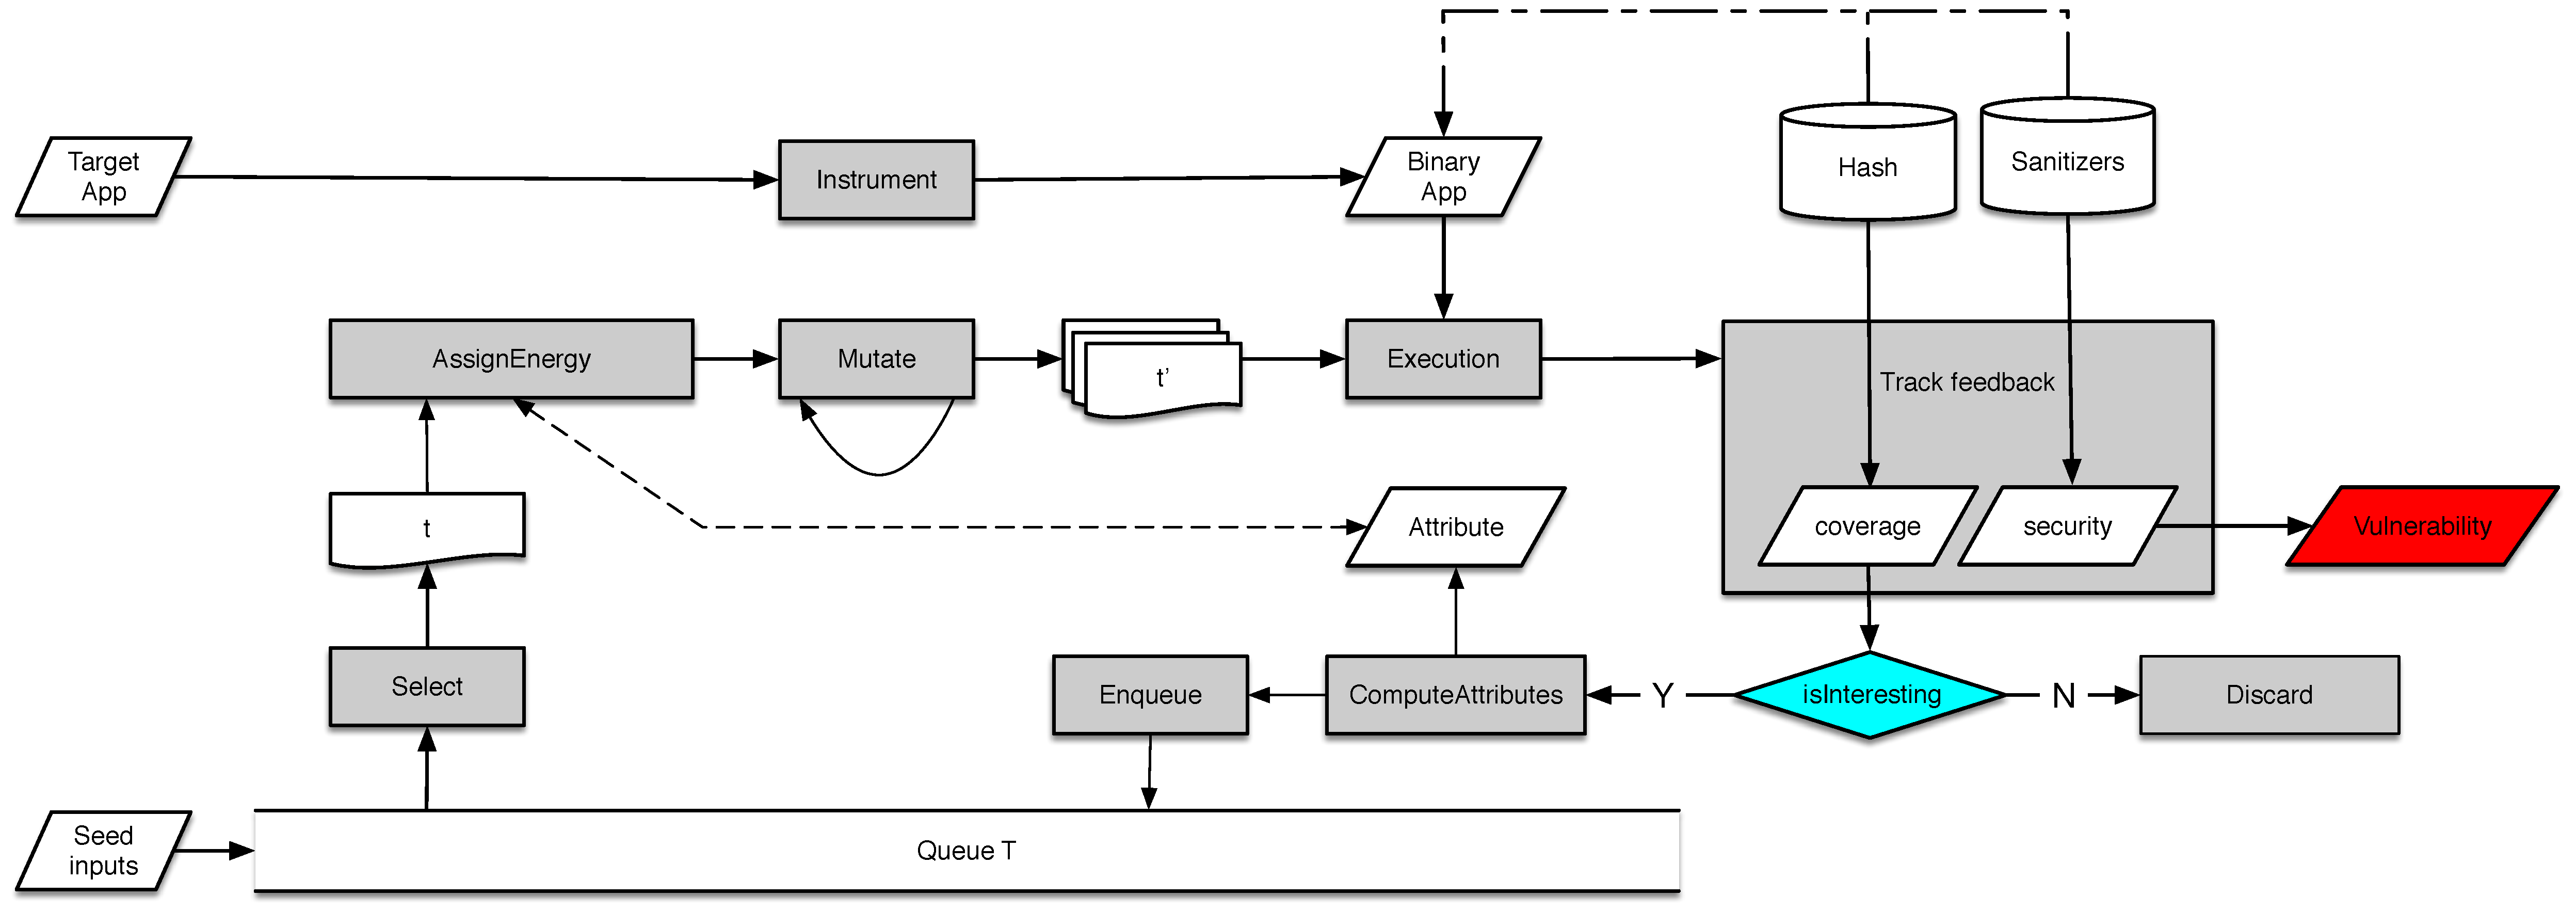
\includegraphics[width=5.5in]{pic/AFL.eps}
%    \caption{The general workflow of AFL  based grey box fuzzing}
%    \label{AFL}
%\end{figure*}
\textbf{Insight 1:} One crucial factor of vulnerability discovery is whether regions that vulnerabilities reside are explored. If vulnerability-residing regions are prioritized and strengthened to be fuzzed, then vulnerabilities could be detected faster and more bugs may be found during same period of time. Existing improvements on guidance are trying to direct fuzzing to reach a specific  location (i.e., the line of code) given in advance, rather than towards promising regions that are more likely for a vulnerability to reside. There are some understanding that sensitive regions(i.e., regions which contain more memory or string operators), complex regions (i.e. code regions with high complexity), deep regions, and rare-reach regions of a program may have more chance to be vulnerable. Thus, guided fuzzing through optimized energy distribution towards these promising vulnerable regions could improve fuzzers' efficiency and detect more bugs. 

\textbf{Insight 2:} Existing energy distribution strategies only tune the mutation number, and randomly select mutation operators.
Empirical studies have shown that coarse-grained mutators (e.g., extra mutators) have better ability to generate diversity test cases, which is helpful for path growth, while fine-grained mutators tend to perform better in exploring nearby execution paths.
Therefore, a better strategy is to adjust the proportion of different granularity mutation operators over time. If certain kinds of mutators perform better, we increase the ratio of these mutators, and vice versa.

\textbf{Key Observation:} Both insight 1 and insight 2 imply that energy distribution matters in greybox fuzzing.

\textbf{Problem Statement:} How to leverage the two insights to improve existing energy distribution strategies and improve the efficiency of AFL based greybox fuzzers?

\textbf{Our Work:} We leverage the two new insights to improve existing AFL's fuzzing energy distribution in a principled way. We direct fuzzers to stress fuzzing toward regions that are more likely for a vulnerability to reside based on static semantic metrics of target program. More specifically, four kinds of promising vulnerable regions (i.e., sensitive, cpmplex, deep and rare-reach regions) are evaluated. And a granularity-aware scheduling of different mutation operators is proposed. The ratio of certain kinds of mutation operators is increased gradually, if they have better ability to trigger new paths. All improvements are integrated and implemented into an newly developed open source fuzzing tool named TAFL. Large-scale experimental evaluations have shown effectiveness of each improvement and the integration. Furthermore, TAFL helps us find five unknown bugs and one new CVE in Libtasn1-4.13\cite{bugs}.

In summary, contributions of our work are as follows:

\begin{itemize}
    \item \textbf{Insights.} We provide two new insights into the energy distribution of AFL based greybox fuzzing.
    
    \item \textbf{Improvements.} We improve the energy distribution strategy in a principled way by leveraging two new insights. More specifically, we improve guidance by directing fuzzing toward four kinds of promising vulnerable regions, and scheduling of different kinds of mutation operators.
    
    \item \textbf{Tool.} We implement and integrate our improvements into a new fuzzing tool named TAFL, which could be accessible from: 
              \url{https://sites.google.com/view/tafl/tool}.
    
    \item  \textbf{Vulnerabilities.} We perform large-scale experimental evaluations to show effectiveness of each improvement and performance of integration. Furthermore, TAFL helps us to find five unknown bugs and one new CVE in Libtasn1-4.13.

\end{itemize}

The remainder of this article is structured as follows: Section \ref{background} is the introduction of American Fuzz Lop (AFL). Section \ref{newinsight} explains our new insights of existing AFL's energy distribution.  Section \ref{approach} gives details of the improvements method by leveraging two insights. Section \ref{impl} describes implementation details. Section \ref{experiment} is the experimental evaluation of each improvement and performance of integration. Section \ref{relatedwork} states related works. Finally, we conclude our work in Section \ref{conclusion}. 









\section{American Fuzzy Lop} \label{background}
AFL based greybox fuzzing is our focus in this paper. AFL based fuzzing tools employ lightweight instrumentation to collect runtime coverage feedback to facilities fuzzing. AFL\cite{afl} and its variations like AFLFast\cite{bohme2016aflfast}, FairFuzz \cite{fairfuzz}, AFLGo \cite{bohme2017aflgo}, CollAFL \cite{gancollafl}, Angora \cite{chen2013angora} are state-of-art AFL based greybox fuzzers. 

%
%\begin{figure*}[t]
%    \centering
%    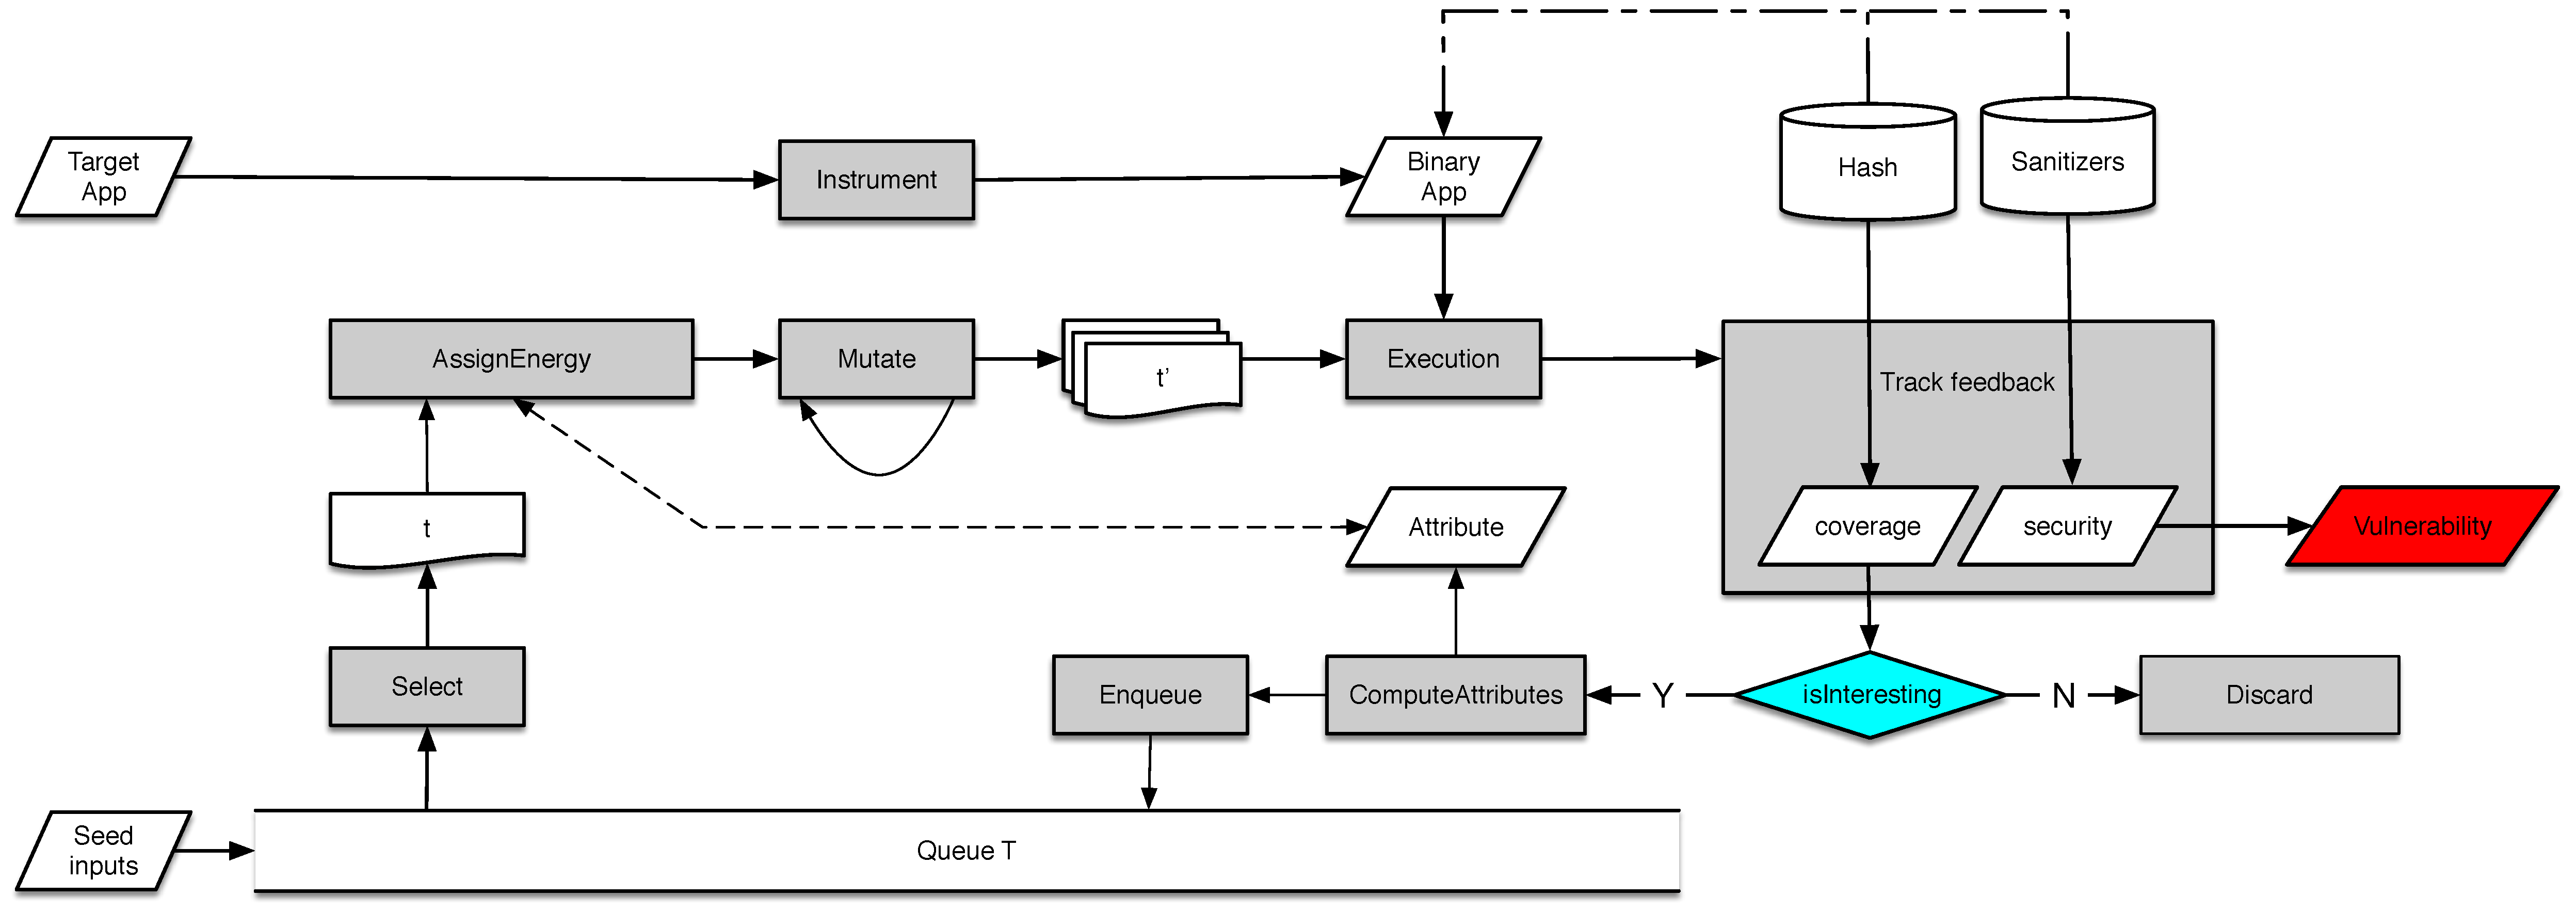
\includegraphics[width=6in]{pic/AFL.eps}
%    \caption{The general workflow of AFL  based greybox fuzzing}
%    \label{AFL}
%\end{figure*}


After instrumenting target program, AFL executes it with some initial seeds. Then, it maintains a queue of test cases and performs an evolutionary fuzzing loop as below:
\begin{enumerate}
\item \textbf{Selecting Seed:} select seed that worth fuzzing from testcase queue with a specific policy (e.g., according to execution time, seed length, and hit number); 
\item  \textbf{Assigning Energy:} calculate and assign energy for selected seed based on its attributes (e.g., execute time, bitmap size, etc.), where the energy of a seed represents number of new test cases that generated from the seed by mutation; 
\item  \textbf{Mutating Input:} mutate seeds using different kinds of mutation operators to generate a batch of new test cases;
\item  \textbf{Executing Target:} feed these new test cases to target application and execute them at a high speed as possible;
\item  \textbf{Tracking Feedback:} track run-time feedback including code coverage, security violation and so on. Meanwhile, vulnerabilities are reported if security violations are detected.
\item  \textbf{Filtering Testcase}: compute and update attributions of testcases, put those good testcases that contributing to code coverage into seed queue, and go to step 1).
\end{enumerate}


Following above continuous evolutionary loop, AFL could generate optimized seeds that explore new execution paths, and thus evolve towards a higher code coverage. As a result, the probability to trigger crashes is increased. The main concepts of AFL fuzzing is described in the following:
 
\subsection{Instrumentation} 

AFL's instrumentation captures basic block transitions, along with coarse branch-taken hit counts. A sketch of the code that shows in listing \ref{instrument} is injected at each branch point in the program. 

\begin{lstlisting}[ frame=single, label= instrument, basicstyle=\small, caption= AFL's Instrumentation]  
cur_location = <COMPILE_TIME_RANDOM>; 
shared_mem[cur_location ^ pre_locatiom] ++;
pre_location = cur_location >> 1;
\end{lstlisting}
The variable $cur\_location$ identifies current basic block. Its random identifier is generated at compile time. Variable $shared\_mem[]$ is a 64 KB shared memory region. Every byte that is set in the array marks a hit for a particular tuple  $(A, B)$ in the instrumented code, where basic block $B$ is executed after basic block $A$. The shift operation in Line 3 preserves the directionality [(A, B) vs. (B, A)]. A hash over $shared\_mem[]$ is used as path identifier. AFL uses coverage information to decide which generated input to retain for fuzzing. Also decides which input to be the priority choice and how long the input will be fuzzed. 
 
\begin{algorithm}[t]
\caption{AFL Greybox Fuzzing} 
\label{aflalgo}
\hspace*{\algorithmicindent} \textbf{Input}: seeds $S$, program $P$

\hspace*{\algorithmicindent} \textbf{Output}: crashes $Tx$
\begin{algorithmic}[1]
    \STATE $Queue \leftarrow S$ ;
    \WHILE{true} 
        \STATE $t \leftarrow$ \texttt{Select}($Queue$);
        \FOR{$i$  from $0$ to Length($t$)}
            \STATE $t' \leftarrow$ \texttt{DeterministicMutate}($t$, $i$);
            \STATE $runResult \leftarrow$ \texttt{RunProgram}($P$, $t'$);
            \IF{$runResult$ is crash}
                 \STATE \texttt{SaveCrashInfo}($runResult$, $Tx$);
            \ENDIF
    
            \IF{$runResult$ is Interesting}
                \STATE \texttt{AddToQueue}($t'$, $Queue$);
                \STATE \texttt{ComputeAttribute}($t'$);
            \ENDIF
        \ENDFOR    
        \STATE $energy \leftarrow$ \texttt{AssignEnergy}($t$);
        \FOR{$i$  from $0$ to $energy$}
            \STATE $t' \leftarrow$ \texttt{MutateInput}($t$, $i$);
            \STATE $runResult \leftarrow$ \texttt{RunProgram}($P$, $t'$);
            \IF{$runResult$ is crash}
                \STATE \texttt{SaveCrashInfo}($runResult$, $Tx$);
            \ENDIF
    
            \IF{$runResult$ is Interesting}
                \STATE \texttt{AddToQueue}($t'$, $Queue$);
                \STATE \texttt{ComputeAttribute}($t'$);
            \ENDIF
        \ENDFOR    
    \ENDWHILE
\end{algorithmic}
\end{algorithm}


Algorithm \ref{aflalgo} illustrates detailed fuzzing process through AFL's implementation. If AFL is provided with seeds $S$, they are added to the $Queue$. Otherwise, an empty file is generated as a starting point.

\subsection{Selecting Seed}
AFL determines a seed if it is $faverable$ based on its length and execution time. A seed will be marked as $favorable$ if it is the fastest and smallest input for any of the edges it exercises.  In process of selecting seed, these $favorable$ seeds will be selected with priority. Non-favorable seeds will be ignored with random probability.

\subsection{Assigning Energy}
The energy of a seed $t$ refers to number of new test cases that generated from $t$ after applying various mutation operators. In deterministic stage, AFL determines a seed's energy according to its length. And in havoc stage, AFL firstly determines the basis energy based on its execution time and average execution time. Then it updates total energy based on others attributes like block transition coverage(i.e., bitmap\_size), handicap, depth and so on.  

\subsection{Mutating Input}
In the act of mutating input, AFL utilizes some typical mutation operators to modify the initial seed, and generate a batch of new test cases. These mutation operators include Flips, Interesting, Arith, Extra and Splice in the following. In determined stage of mutation, these mutation operators will be used separately and sequentially to generate new test cases; And in havoc stage, AFL would mutate the seed by randomly choosing a sequence of mutation operators and apply them to random locations in the seed file. 

These mutation operators in AFL  are:
\begin{itemize}
\item  \textbf{Flips:} simple bitflip, two bitfilp, four bitflip, etc. 
\item  \textbf{Interesting:} set "interesting" bit, bytes, words, dwords.
\item  \textbf{Arith:} addition or subtraction of bytes, words or dwords.
\item  \textbf{Extra:} block deletion, block insert, overwrite, etc.
\item  \textbf{Splice:} splice two distinct input files at a random location.
\end{itemize}

\subsection{Tracking Feedback}
When a new test case is generated, it is fed to target program and executed by AFL. At run-time, feedback including code coverage and security violation are tracked.  AFL determines an input to be interesting only if that input has contribution to code coverage. Intuitively, AFL retains inputs that invoke a new block transition or a path where a block transition is executed twice while it normally executes only once. If the generated input $t^{'}$ crashes the program, it is added to a set of crashing inputs. A crash input that is also interesting will be marked as a unique crash. 

\subsection{Filtering Testcase}
If the generated input $t^{'}$ is considered to be interesting, AFL will run a calibration stage to compute and update its attributes, then add it into the queue. These attributes are  important because they are the basis for energy assignment. More specifically, these attributes include execution, bitmap, hit numbers and so on.

\section{New Insights}\label{newinsight}
During the process of using AFL based greybox fuzzers (e.g., AFL and AFLFast), we have some new insights about existing AFL's fuzzing energy distribution strategy. In this section, a detailed description of two insights is illustrated.

%\textbf{Insight 1: } Existing energy distribution strategies discriminate against time-consuming (TC) paths, which are usually paths containing long loops.  TC paths are ignored with large probability, and given little energy even if not ignored. At the select stage, AFL will prefer to choose the test case that execute faster and its size is smaller. And at the stage of compute the energy amount, the basis of the energy is determined by its execute time.  The core idea to determine the basis energy is the longer execute time, the smaller energy assigned, the maximize basis is 30 times of minimize basis. The detailed rules is shown in Table \ref{EnergyBasis}.
%\begin{table}[hbpt]
%\centering
%\label{EnergyBasis}
%\caption{Basis Energy Determine Rules}
%\begin{tabular}{|l|}
%\hline
%q $\rightarrow$ exec\_us * 0.10      $>$  avg\_exec\_us    $\rightarrow$  perf\_score = 10; \\
%q $\rightarrow$ exec\_us * 0.25      $>$  avg\_exec\_us    $\rightarrow$  perf\_score = 25;\\
%q $\rightarrow$ exec\_us * 0.50      $>$  avg\_exec\_us    $\rightarrow$  perf\_score = 50;\\
%q $\rightarrow$ exec\_us * 0.75      $>$  avg\_exec\_us    $\rightarrow$  perf\_score = 75;\\
%q $\rightarrow$ exec\_us * 2.00      $<$  avg\_exec\_us    $\rightarrow$  perf\_score = 150;\\
%q $\rightarrow$ exec\_us * 3.00      $<$  avg\_exec\_us    $\rightarrow$  perf\_score = 200;\\
%q $\rightarrow$ exec\_us * 4.00      $<$  avg\_exec\_us    $\rightarrow$  perf\_score = 300;\\
%\hline
%\end{tabular}
%\end{table}
%
%Where the $exec\_us$ represent the execute time of the test case $q$, and the $avg\_exec\_us$ represent the average execute time. $perf\_score$ is the score used for assigning energy.
%
%For institution, take following code fragment listed in the Listing \ref{TCPath} as an example to illustrate the discrimination against time-consuming paths. Considering the two paths distinguished by buf[0], there are two same crash bugs (i.e. crash A, crash B)  at the end of each path. The existing AFL's energy distribution  strategy is based on the execution time of the test case, the size of the bitmap and so on. Let the execute time of each instrument be one second. The total execute time of Path A to trigger crash A is 10002s, while the execute time of Path B to trigger crash B 14s, and the bitmap size of path A crash and path B crash is 3 and 7. Then based on the computation formula in AFL, the energy score of Path A maybe 7.5 (i.e. 10 $\times$ 0.75)  and the energy score of path B maybe 450 (i.e. 300$\times $1.5). That means that  the time-saving path (Path B)'s energy is 60 times larger then time-consuming path (Path A). 
%
%This discrimination makes it difficult to detect vulnerabilities buried in TC paths, such as crash A behind long loop. Furthermore, when the execute time is larger than the setting limit time of AFL, it may obtain hang, but never detect these kind of crashes.  Thus, energy assignment should give TC  paths opportunities and energy in order to balance the probabilities to detect bugs in time-consuming and time-saving paths.
%
%\begin{lstlisting}[float, language=C++,caption=Sample code contain Time-Consuming path, label=TCPath]
%#include "stdio.h"
%int main (int argc, char ** argv){
%    char buf[8];
%    if(read(0, buf, 8) < 1){
%        printf("Hum ?\n")
%        exit(1);
%    }
%    
%    if(buf[0] == 'a'){  //Path A
%        char * arr;
%        for(int i = 0; i< 10000; i++){
%               ......    
%        }
%        
%        if(buf[6]=='g' && buf[7]=='h' ){
%            abort();        // crash A
%        }
%    
%    }else if(buf[1]=='b'){   // Path B
%        if(buf[2] == 'c'){ 
%             printf("reach c\n");
%            if(buf[3]=='d'){ 
%                 printf("reach c\n");
%                if(buf[4]=='e'){
%                    printf("reach c\n");
%                    if(buf[5]=='f'){ 
%                        printf("reach c\n");
%                        if(buf[6]=='g' && buf[7]=='h'){  
%                            abort();        // crash B            
%                        }else printf("error\n");                        
%                    }else printf("error\n");                    
%                }else printf("error\n");            
%            }else printf("error\n");    
%        }else printf("error\n");    
%    }
%}
%\end{lstlisting}


\begin{figure}[t]
    \centering
    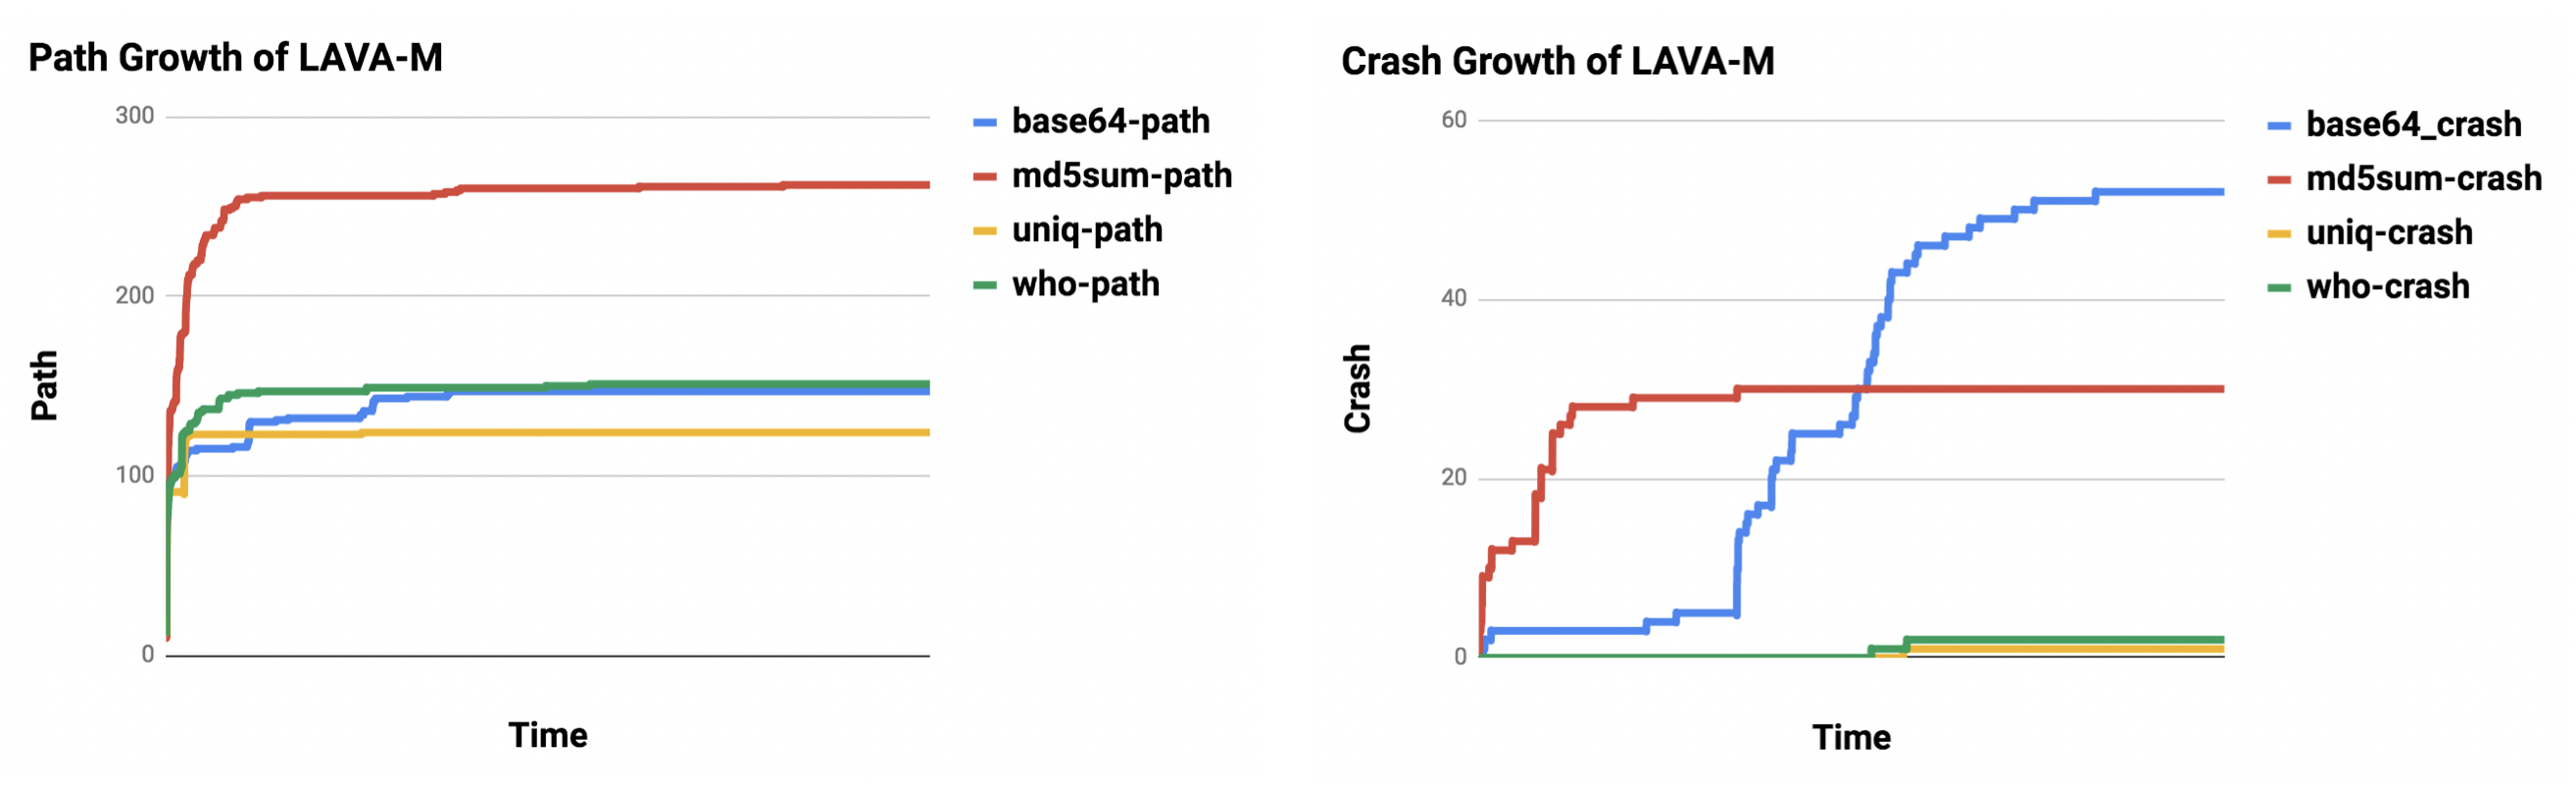
\includegraphics[width=3.5in]{pic/insight11.png}
    \caption{path and crash growth over time}
    \label{path-crash-growth}
\end{figure}
%explain your experimental setup?
%\gl{check the legend on the right: base64})

\textbf{Insight 1: } Growth of paths follows the same pattern, while growth of crashes has no definite rules. The Fig.\ref{path-crash-growth} is a statistical result of path growth and crash growth of LAVA-M \cite{lava} benchamrk fuzzed by AFL. As shown in Fig.\ref{path-crash-growth}, number of total path increases quickly at the beginning, and growth rate gradually becomes flat over time. Finally, it will become harder to find new path. And slop of growth curve is approximating zero. A natural reason is that discovery of new path is a Coupon Collector’s Problem (CCP) \cite{ferrante2014coupon}. After finding $i-1$ new paths, the probability of finding the $i$th new path is $P_{i}= (N-i+1)/N$, where $N$ is the number of total paths. From this formula, we can see that the discovery of new paths is increasingly difficult over time. Compared with path growth pattern, occurrence and increment of crashes are completely different. There is no universal model for the emergence and growth of crashes. As can be seen from above Fig. \ref{path-crash-growth}, crash may appear very early. It also may occur very late. Crash may grow faster at the beginning and then not grow later. It also may not grow at first, and then grow faster later. The reason behind this phenomenon is that direct cause of crash discovery is not increment of path coverage, but whether regions where vulnerabilities resided are explored. 

%
%\begin{lstlisting}[float, language=C++,caption=Sample code of energy distribution, label=DirectPath]
%#include "stdio.h"
%int fun (const uint8_t *Data, size_t Size, bool e){
%   if(e = true && Size ==22){                  // Path A
%      uint64_t x = 0;
%      int64_t  y = 0;
%      int32_t z = 0;
%      uint16_t a = 0;
%      memcpy(&x, Data, 8);  
%      memcpy(&y, Data + 8, 8);  
%      memcpy(&z, Data + 16, sizeof(z));  
%      memcpy(&a, Data + 20, sizeof(a));  
%     
%      if(x = 10 && y == 0xbaddcafedeadbeefUL)
%             abort();       
%       
%  }else if (e == false && Size < 22){    // Path B
%     printf("%d\n", *Data);
%      uint64_t x = 0;
%      memcpy(&x, Data, 8);  
%      if(x>10)
%          abort();
%  }
%}
%\end{lstlisting}

If those regions that are more likely for a vulnerability to reside are prioritized and strengthened to fuzz, related vulnerabilities buried in these regions will be detected faster. Furthermore, more bugs could be found during the same period of time. 

There are some common intuitions that sensitive region(i.e. region containing much memory or string related operators), complex region, deep region, and rare-reach region are more likely to be vulnerable due to developer negligence and inadequate testing. Thus, guide fuzzing toward these promising vulnerable regions and spend more fuzzing energy on them will improve the efficiency of fuzzing tool. 
%\gl{why is sensitive region prone to vulnerabilities? The rest are institutive, not sensitive region.}


%For the institution, take the following code fragment listed in the Listing \ref{DirectPath} as an example to show the rationality of promising area deserve more energy. Considering the path A and path B in Listing \ref{DirectPath}, path A contains more sensitive instruments like memcpy(). Also, it is more complicated than path B for it contains more instruments, and the bug is located deeper and rare-to-reach. Then we should spend more energy on Path A, no matter if there are bugs or not.
%
%Thus,  directed fuzzer prioritize fuzzing these vulnerability-promising areas and spend more fuzzing energy on these areas will improve the efficiency to detect vulnerabilities. 


\textbf{Insight 2: } Existing energy distribution strategy only considers calculation of mutations numbers. It does not consider scheduling of distribution ratio of different kinds of mutation operators. The energy refers to the number of new test cases generated by mutating seed using various granularity mutation operators. It is calculated based on seed's attributes such as execution time, bitmap size, depth, hit numbers and so on. However, scheduling of distribution proportion for different kinds of mutation operations in assigned number does not get enough attention it deserves. In determined stage of mutation, AFL applies mutation operators (e.g., Flips, Interesting, Arith, Extra, and Splice) separately and sequentially to generate new test case; And in havoc stage, AFL would mutate the seed by randomly choosing a sequence of different mutation operators and apply them to random locations in the seed files. 

\begin{figure}[t]
    \centering
    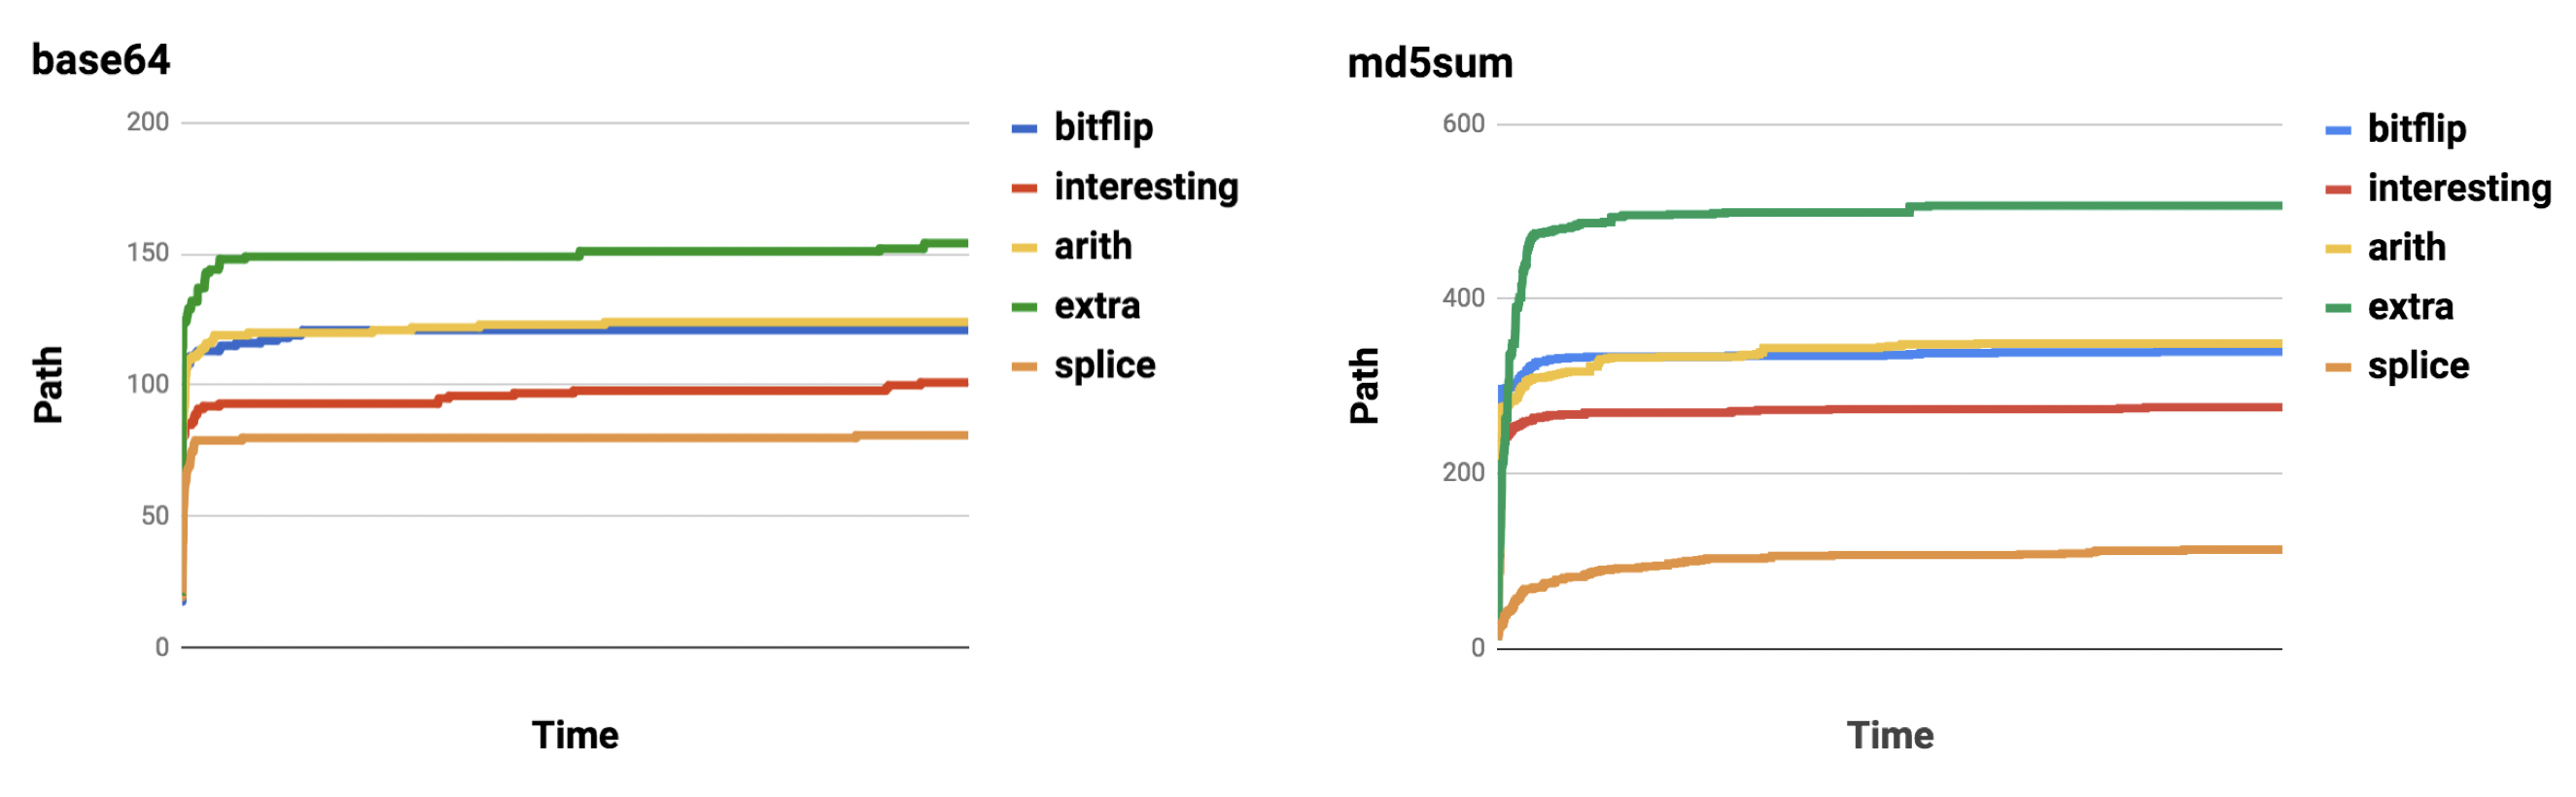
\includegraphics[width=3.5in]{pic/insight22.png}
    \caption{path growth using different mutators }
    \label{FineCoarseEffect}
\end{figure}

Experimental evaluation of each kind of mutation operators are performed on LAVA-M \cite{lava}, and the results are listed in Fig. \ref{FineCoarseEffect}. It indicates that different mutators have different abilities to trigger new path. Extra mutations have better ability to generate diversity test case, which is more helpful to the path growth. On the other hand, splice mutators perform poor. (2) The effect of combining multiple kinds of mutators is better than the effect of using single kind of mutator.% (3) The coarse-grained mutators are better than fine-grained mutators on helping path growth. 
However,  randomly choosing mutators without scheduling may cause overuse of some low effective mutation operators, and lack of diversity.


Thus, the energy distribution should consider not only the number of mutations but also the proportion of different kinds of mutation operators in assigned number. Despite the fact that finding new path will become more and more difficult, the proportion of mutation operations who has better ability to trigger new paths should gradually increase over time.


 


%\section{Methodology}\label{Methodology}

\subsection{Feedback fuzzing as Markov Decision Process}

\begin{figure}[t]
	\centering
	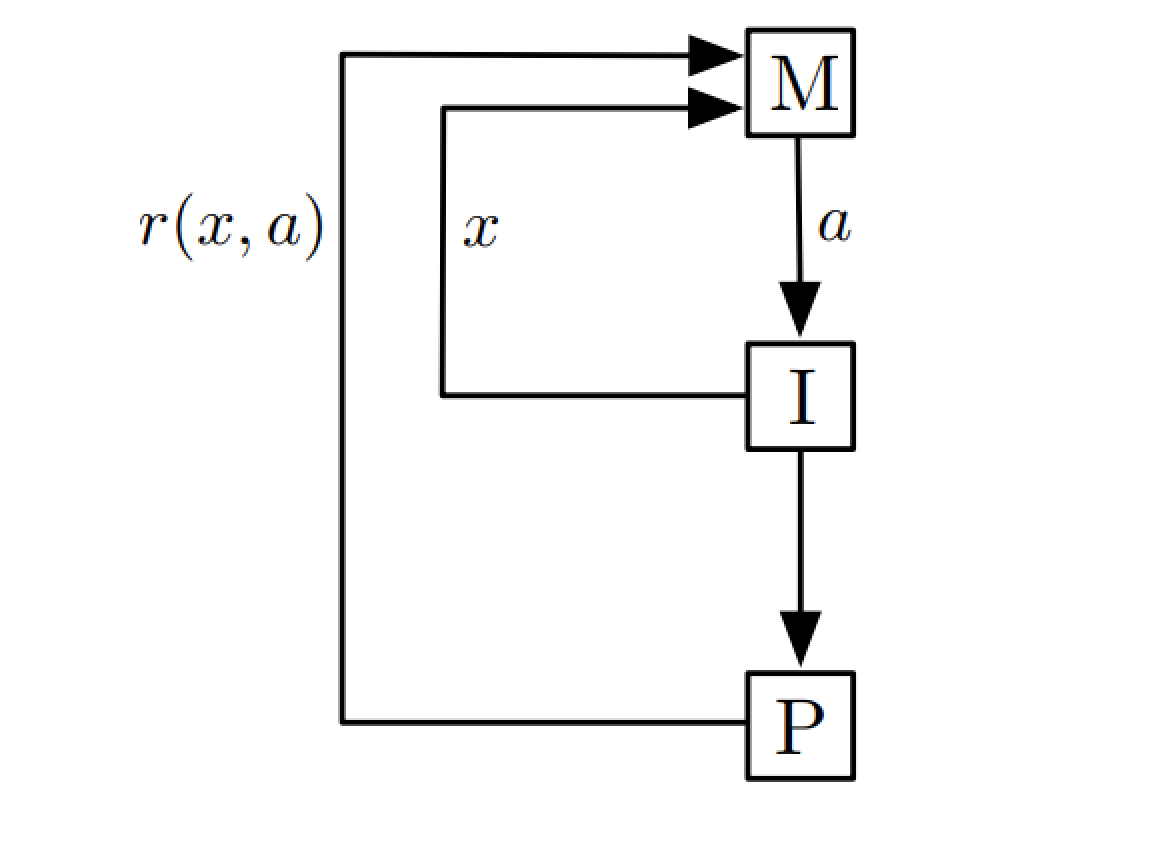
\includegraphics[width=2in]{pic/modeling.png}
	\caption{Feedback fuzzing as Markov Decision process}
	\label{modeling}
\end{figure}

Feedback based fuzzing can be modeled as learning process with a feedback loop. Initially, the fuzzer generates new inputs, and then runs the target program with each of them. For each program execution, the fuzzer extracts runtime information (gathered for example by binary instrumentation) for evaluating the quality (with respect to the defined search heuristic) of the current input. For instance, this quality can be measured as the number of (unique or not) instructions executed, or the overall runtime of the execution. By taking this quality feedback into account, a feedback-driven fuzzer can learn from past experiments, and then generate other new inputs hopefully of better quality. This process repeats until a specific goal is reached, or bugs are found in the program. Similarly, the reinforcement learning setting defines an agent that interacts with a system. Each performed action causes a state transition of the system. Upon each performed action the agent observes the next state and receives a reward. The goal of the agent is to maximize the total reward over time.

An input mutator engine M generates a new input I by performing a fuzzing action a, and subsequently observes a new state x directly derived from I as well as a reward r(x,a) that is measured by executing the target program P with input I.

More specificlly, we using formaluate the feedback greybox fuzzing as Markov decision process by defining states, action, and reward in the fuzzing context.

\subsubsection{States}
We consider the system that the agent learns to interact with to be a given "seed" projram input. Further, we define the states that the agent observes to be substrings of consecutive symbols within such an input. Formally, let $\sum$ denote a finite set of symbols. The set of possible program inputs $I$ written in this alphabet is then defined by the Kleene closure $I : = \sum^{*}$. For an input string $x = x_{1}, ..., x_{2} \in I$, let
$$S(x) := {(x_{1+i}, ..., x{m+i} | i\geq 0, m+n \leq n)}$$
denote the set of all substrings of x. Clearly, $\cup_{x\in I}S(x) = I$ holds. We define the states of out Markov decision process to be $I$. In the following, $x\in I$ denotes an input for the target program and $x^{'} \in S(x) \subset I$ a substring of this input..

\subsubsection{Actions}
We define the set of possible actions $A$ of our Markov decision process to be random variables mapping substrings of an input to probabilistic rewriting/ mutation rules:

$$A:={a:I \rightarrow (I \times I, F, P)|a~\pi(x^{'})}$$

where $F = \sigma (I \times I)$ denotes the $\sigma$-algebra of the sample space $(I \times I)$ and P gives the probability for a given rewrite rule. In our Implementation, we define a small subset $A \subset A$ probabilistic string rewrite rules that operate on a given seed input.

\subsubsection{Rewards}
We define rewards independently for both characteristics of (1): the next preformed action $a$ and (2) the program execution with the next generated input x, i.e. $r(x,a)$= $E(x)$+$G(a)$.
In our implementation, we experiment with E providing the numbers of newly discoverd bsic blocks, execution path length,  and execution time of the target that processes the input x. For example, we can define the number of newly discovered blocks as 
$$E_{1}(x, I^{'} := |B(c_{x} \setminus) (\cup_{x\in I^{'}}B(c_{x}))|)$$
where $c_{x}$ denotes the execution path the target program takes when processing input x, $B(c_{x})$ is the set of unique basic blocks of this path, and $I^{'} \subset I$ is the set of previously processed inputs. Here, we define a basic block as a sequence of program instructions without branch instructions.

\subsection{Guided feedback fuzzing as Reward optimization problem}

Now we modeling the feedback greybox fuzzing as the Markov decision process. Furthermore, the  guided feedback greybox fuzzing could be cast into objected optimization problem. The object is to maximize the feedback reward.

The official AFL exploit the qualitative reward feedback, i.e. if the test case trigger new block to block transition) to saving interesting test case and mutate it to achieve the goal of coverage more new branch. AflFast use the quantitative reward(branch hit number) as reward to mutate more test case based on test case that trigger low frequency path, its goal is also to maximize the code coverage more efficiency.

Beside the goal of maximize the coverage,  we could achieve other optimization object by choosing highly-rewarded actions and spending more resource on the highly-reward actions.

For example, if the feedback reward is the quantitative depth of execution path. Based on our institution that the deeper we explore, the more change we could find vulnerabilities. Our guided fuzzing goal maybe to reach the deepest path as soon as possible, then we could choose and spend more resource on those test case that explore deeper.

If the feedback reward is the quantitative complex degree of execution path, and based on institution that the more complex area, the more chance to be vulnerable. Our goal of guided fuzzing maybe to explore the most complex path as soon as possible, then we could choose and spend more resource on these test cast that explore more complex path.

If the feedback reward is the connection degree from its neighborhood of the execution path, and based on our institution that if the connection degree is lesser, the fair reach of these area, and the fairer to reach, the more chance to have bugs in these fair reach areas. Our goal of guided fuzzing maybe to execute the most fair reach areas as soon as we can. Then we could choose and spend more resource on these test case that explore  fairer reach areas.

So far, we  cast the goal guided feedback fuzzing as the object optimization problem to achieving the highest reward as soon as possible.

\subsection{Fish School Search based Energy Scheduler}

Now we have the goal like exploring the deepest path, the most complex path, the fairest reach path as soon as possible. And we know where to spend more resource according to the different goals. If our goal is to execute the deepest, we will chose the test case that executed deeper path, and spend more resource on the test case (specify we mutate more test case based on the test case.)

Then we know we should spend more resource on these test case that its reward is higher, and the higher the reward, the more resource we should spend. But how much more resource is spent is another balance problem.

We borrow the ideas of movement operators from fish school search algorithm. The core idea is to make the fishes “swim” toward the positive gradient in order to “eat” and “gain weight”. Collectively, the heavier fishes are more influent in the search process as a whole, what makes the barycenter of the fish school moves toward better places in the search space over the iterations.

Similarly, we model the execution of one test case as swim of one fish,  and reward it obtain along the path is regarded as "weight", the heavier test case will have more in influence and attract more resource. Then other fishes(test cases) will follow the heavier fish. We modeling the resource distribution as the movement operators of fish school search algorithm.


We design three strategies of quantitative resource distribution : constant, linear, exponential and sqrt.

If the total reward of each execution of one test case is donated as $TotalReward(T) = \sum Reward(BB_{i})$ where, $BB \in Path(T)$. We update the Maximize path weight,  Minimize path weight, and calculate the average path weight (i.e. $AvgPathWeight= MaximinzePath + MinimizePath /2$) as the \textbf{KEY } parameter for energy assignment.




\section{Improvements} \label{approach}
Two new insights were leveraged to improve the fuzzing energy distribution strategy in a principled way. The improvements contain two aspects: (1) improvement of directing fuzzing toward promising regions that are more likely to have vulnerabilities; and (2) improvement of scheduling of the distribution ratio of different mutation operators.  Finally,  these improvements are organically integrated and implemented into a new tool.

%\subsection{Improvement of balance to time-consuming paths}
%As shown in insight 1, existing energy assignment formulas discriminate against time-consuming procedures. More specific, the AFL(including AFLFast)  will prefer time-saving test case and assign the basis energy based on execute time as Table \ref{EnergyBasis}. The strategy of AFLFast prefer low frequence path and spend more energy on low frequence path, this measure has effect on reduce the discrimination on TC path, but it will lead to strut on TC path sometime, and the basis energy calculation is same as AFL. We try to balance  fairness for TC path with the execute speed of fuzzers. So we change the basis energy calculation using with a specific probilities.  We will using Rule listed in Table \ref{EnergyBasis} with 70\% probilities, and using Rule listed in Table 2 with 30\%.
%
%\begin{table}[hbpt]
%\centering
%\label{EnergyBasis2}
%\caption{Basis Energy Determine Rule2}
%\begin{tabular}{|l|}
%\hline
%q $\rightarrow$ exec\_us * 0.10      $>$  avg\_exec\_us    $\rightarrow$  perf\_score = 300; \\
%q $\rightarrow$ exec\_us * 0.25      $>$  avg\_exec\_us    $\rightarrow$  perf\_score = 200;\\
%q $\rightarrow$ exec\_us * 0.50      $>$  avg\_exec\_us    $\rightarrow$  perf\_score = 150;\\
%q $\rightarrow$ exec\_us * 0.75      $>$  avg\_exec\_us    $\rightarrow$  perf\_score = 75;\\
%q $\rightarrow$ exec\_us * 2.00      $<$  avg\_exec\_us    $\rightarrow$  perf\_score = 50;\\
%q $\rightarrow$ exec\_us * 3.00      $<$  avg\_exec\_us    $\rightarrow$  perf\_score = 25;\\
%q $\rightarrow$ exec\_us * 4.00      $<$  avg\_exec\_us    $\rightarrow$  perf\_score = 10;\\
%\hline
%\end{tabular}
%\end{table}
% 
%
%And at early stage, we follow the energy assignment of original AFL, and when the path growth become flat, we prefer to make the time-consuming test case as favorable, and spend more energy. 

\subsection{Improvement of Directing Toward Promising Regions}
Inspired by AFLGo, which directs fuzzing to reach some specific code lines. We improve the guidance of AFL toward promising vulnerable code regions. The core idea is to extract semantic metrics of basic blocks of target program using light-weight Intermediate representation (IR) level static analysis. Then we instrument these qualitative weights into original program through compiler-time instrumentation. At run-time, path reward (i.e., sum of weight) is traced. If a test case is interesting, we assign energy based on its path reward. The seeds who win more rewards will be assigned with more energy. In this way, based on specific semantic metrics of code region, fuzzing could be directed to stress fuzzing those promising vulnerable regions, like sensitive regions, complex regions, deep region and rare-reach regions. 

We demonstrate an Intuitive example to explain energy assignment using the abstract control flow graph (CFG) shown in Fig.\ref{cfg}. 

\begin{figure}[t]
\centering
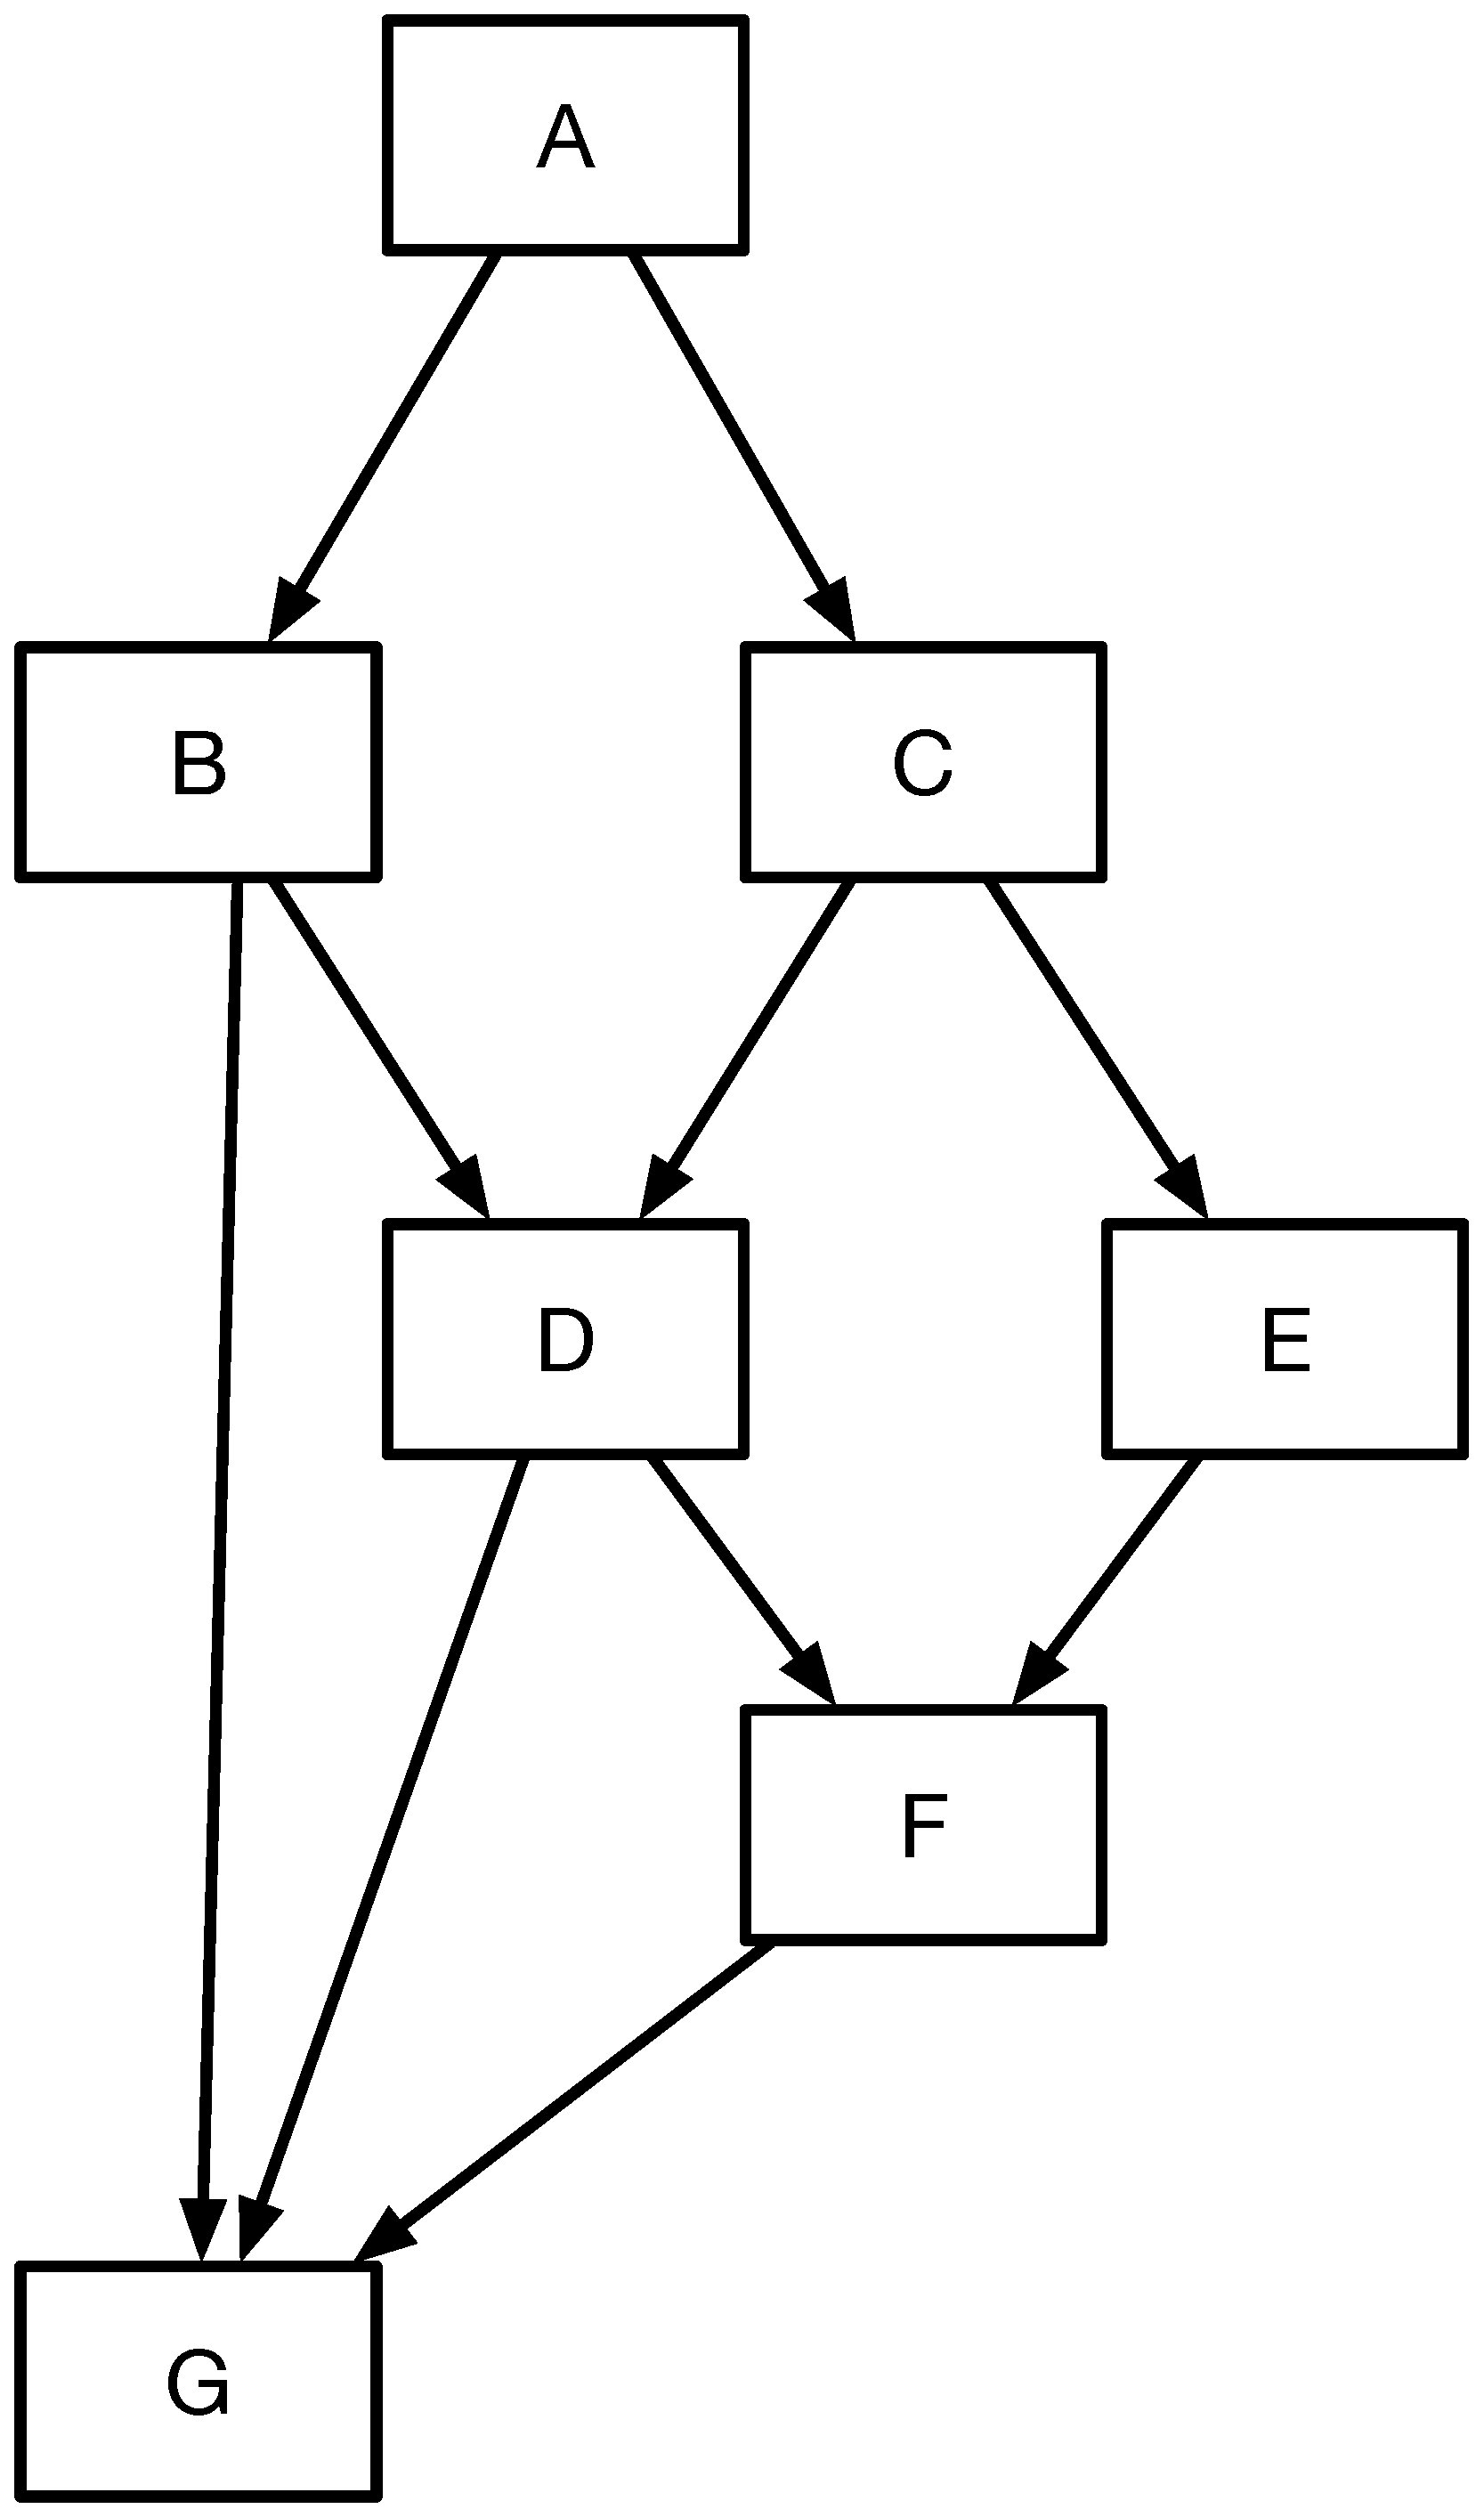
\includegraphics[width=1in]{pic/AbstractCFG.eps}
\caption{Abstract CFG}
\label{cfg}
\end{figure}

Let weight of a basic block $BB$ for a specific $metric$ be $weight_{metric}(BB)$. Then, reward of a path that executed with input $t$ could be denoted as:
\begin{equation}
Reward(t)=  \frac{\sum_{i=0}^{n} weight(BB_{i})}{n}, BB_{i} \in path(t)
\end{equation}

Sum of block weights in path $path(t)$ exercised by the input $t$ is counted. Note that we count the basic blocks in loop for multiple times. Intuitively, if test case $t$ executes the path of $p= A \rightarrow B \rightarrow D \rightarrow G$, then $Reward(t)$=$(weight_{metric}(A)$ + $weight_{metric}(B)$ + $weight_{metric}(D)$ + $weight_{metric}(G) )/4$. After an execution is finished,  the maximum, minimum reward and average reward are updated. Average reward $AvgReward$ is calculated using equation as shown below:
\begin{equation}
 AvgReward = \dfrac{MaxReward + MinReward} {2}
 \end{equation}
 
Furthermore, $Factor$ used for energy assignment is computed based on a seed's reward and average reward value. 
 \begin{equation}
Factor(t)= \dfrac{Reward(t)}{AvgReward}
 \end{equation}

$Factor$ affects the amount of energy assignment. The bigger the $Factor$ is, the more energy is assigned.  More specifically, an exponential energy assignment formula in the following is used to assign energy based on the $Factor$. Let $P_{afl}(t)$ be the energy assigned by AFL for input $t$, and energy $P(t)$ for test case $t$ assigned after improvement could be donated as following:
\begin{equation}
P(t) = P_{afl}(t) * 2^{ 10 * Factor(t)}
\end{equation}

Thus, based on institutions that the more sensitive, complex, deeper and more rarely reachable regions, the more chance to be vulnerable. Four kinds of related semantic metric are designed and used to drive fuzzing. The four kinds of semantic metric represents four kinds of promising vulnerable regions. They are sensitive region,  complex region, deep region, and rarer-reach region. Note that our metrics are one possible representation of four kinds of regions, the four regions could also be represented using other metrics.

\subsubsection{Towards Sensitive Region}
According to the intuition that if a path contains more sensitive operators like memory and string related instruments, it is more likely to occur memory corruption vulnerabilities.  Thus, a sensitive metric is designed to measure the sensitive degree of the code region (i.e., basic block). More specifically, measurement of sensitive metric is defined as follows:
\begin{equation}
SensitiveDegree(BB) =MemoryOP + StringOP
\end{equation}

Where, $SensitiveDegree$ represents the total numbers of memory and string related instruments in the basic block $BB$. 

\subsubsection{Toward Complexity Region}
Based on intuition that more complex areas are more likely to have vulnerabilities, complexity metric are designed to measure complexity of each basic block. The number of total instruments in a basic block is a simple and direct indicator to show the complexity of a code region. Thus, we used instrument number as the complex metric, and the measurement is as follows:
\begin{equation}
ComplexityDegree(BB) ={InstNum}
\end{equation}

where $ComplexityDegree$ represents the total numbers of instruments in basic block $BB$. 


\subsubsection{Toward Deep Region}

Based on intuition that it has more chance to detect vulnerability by exploring the deep path,  we define depth metric to show the deep degree of a path. It represents the distance from the function's entry block to the basic block itself. More specifically, the measurement of depth metric of basic block $BB$ as follows:

For a given basic block $BB$, all the paths $P$ that from entry block $E$ within function to the basic block $B$ are traversed, which is donated by $P=path(E,BB)$. Assume the depth of path $p_{i} \in P$ is $d_{i}$, then depth of $BB$ is as follows equation:
\begin{equation}
Depth(BB)= \dfrac{1}{ \sum_{p_{i} \in P}  \dfrac{1}{d_{i}}}
\end{equation}

Intuitively,  take Fig. \ref{cfg} as an example, to calculate depth of basic block $G$, the abstract CFG is traversed using deep first search (DFS) algorithm. And paths from entry block $A$ to $G$ are obtained firstly. They are $p_{1}=A\rightarrow B\rightarrow G$, $p_{2}=A\rightarrow B\rightarrow D\rightarrow G$,  $p_{3}=A\rightarrow C\rightarrow D\rightarrow G$, $p_{4}=A\rightarrow B\rightarrow D\rightarrow F \rightarrow G$, $p_{5}=A\rightarrow C\rightarrow D\rightarrow F \rightarrow G$, $p_{5}=A\rightarrow C\rightarrow E\rightarrow F \rightarrow G$.  The length of above paths are 2, 3, 3, 4, 4. ( i.e. $l_{p_{1}} = 2$, $l_{p_{2}}=3$, $l_{p_{3}}=3$, $l_{p_{4}}=4$ , $l_{p_{5}}=4$). Then, depth of basic block $G$ is computed as equation (7), and result is $1/(1/2 + 1/3 + 1/3 + 1/4 + 1/4) = 3/5$. Note that computation of depth is based on intra-procedure static analysis without considering function-level distance. It may sacrifice certain accuracy for conveniences of usage.

\subsubsection{Toward Rare-Reach Region}

Based on intuition that if a code region has lower reachable probability, the region may have higher chance to have issues. The reason behind this intuition is that rare-reach areas are usually not suffering from sufficient testing, especially in integration testing phase. Thus, metric called $RareReachDegree$ is defined to represent the rarely reachable degree of a region (i.e., basic block of program). More specifically, measurement of rarely reachable degree is calculated as follows.

For a given basic block $BB$, the probability to all its outgoing edges are assumed to be equal. Hence, if $succ(BB)$ denotes number of all successor basic blocks of $BB$, then $\forall b \in succ(BB)$, $TPro(B, b)$ = 1 / $succ(B).size$, where $succ(B).size > 0$.  All paths $P$ that from entry block $E$ of function to basic block $BB$ itself are traversed, and denoted by $P=path(E, BB)$.

Given a path $p_{i} \in P$, the reachable probability of $BB$ in path $p_{i}$ is calculated using below equation:
\begin{equation}
RPro(BB,p_{i})=\dfrac{1}{\prod_{j=0}^{p_{i}.size -1} TPro(B_{j}, B_{j+1})} 
\end{equation}

Furthermore, we will calculate all paths and finally get the rarely reachable degree of basic block $BB$ as follows:
\begin{equation}
RareDegree(BB)= \dfrac{1}{ \sum_{i=0}^{P.size - 1} RPro(BB, p_{i})}
\end{equation}

Similarly, take Fig.4 as an example for sake of clarity. In order to compute depth of basic block $G$, we will traverse the control flow graph using DFS algorithm and get all the paths from entry block $A$ to basic block $D$. They are $p_{1}=A\rightarrow B\rightarrow D$, $p_{2}=A\rightarrow C\rightarrow D$.  Then,  rare-reach degree of $B$ is calculated using equation (8) and (9), and the result is $1/(1* 1/2 + 1 *1/2) = 4$. 


\subsection{Improvement of Schedule of Mutators}
Existing energy assignment strategies only consider number of mutations. But they do not take into account the distribution of different granularity mutation operations in assignment number. In order to add flexible granularity-aware scheduling for different kinds of mutation operations, an understanding of different granularity mutation operators' abilities to promote path growth is needed firstly.

\begin{figure}[t]
    \centering
    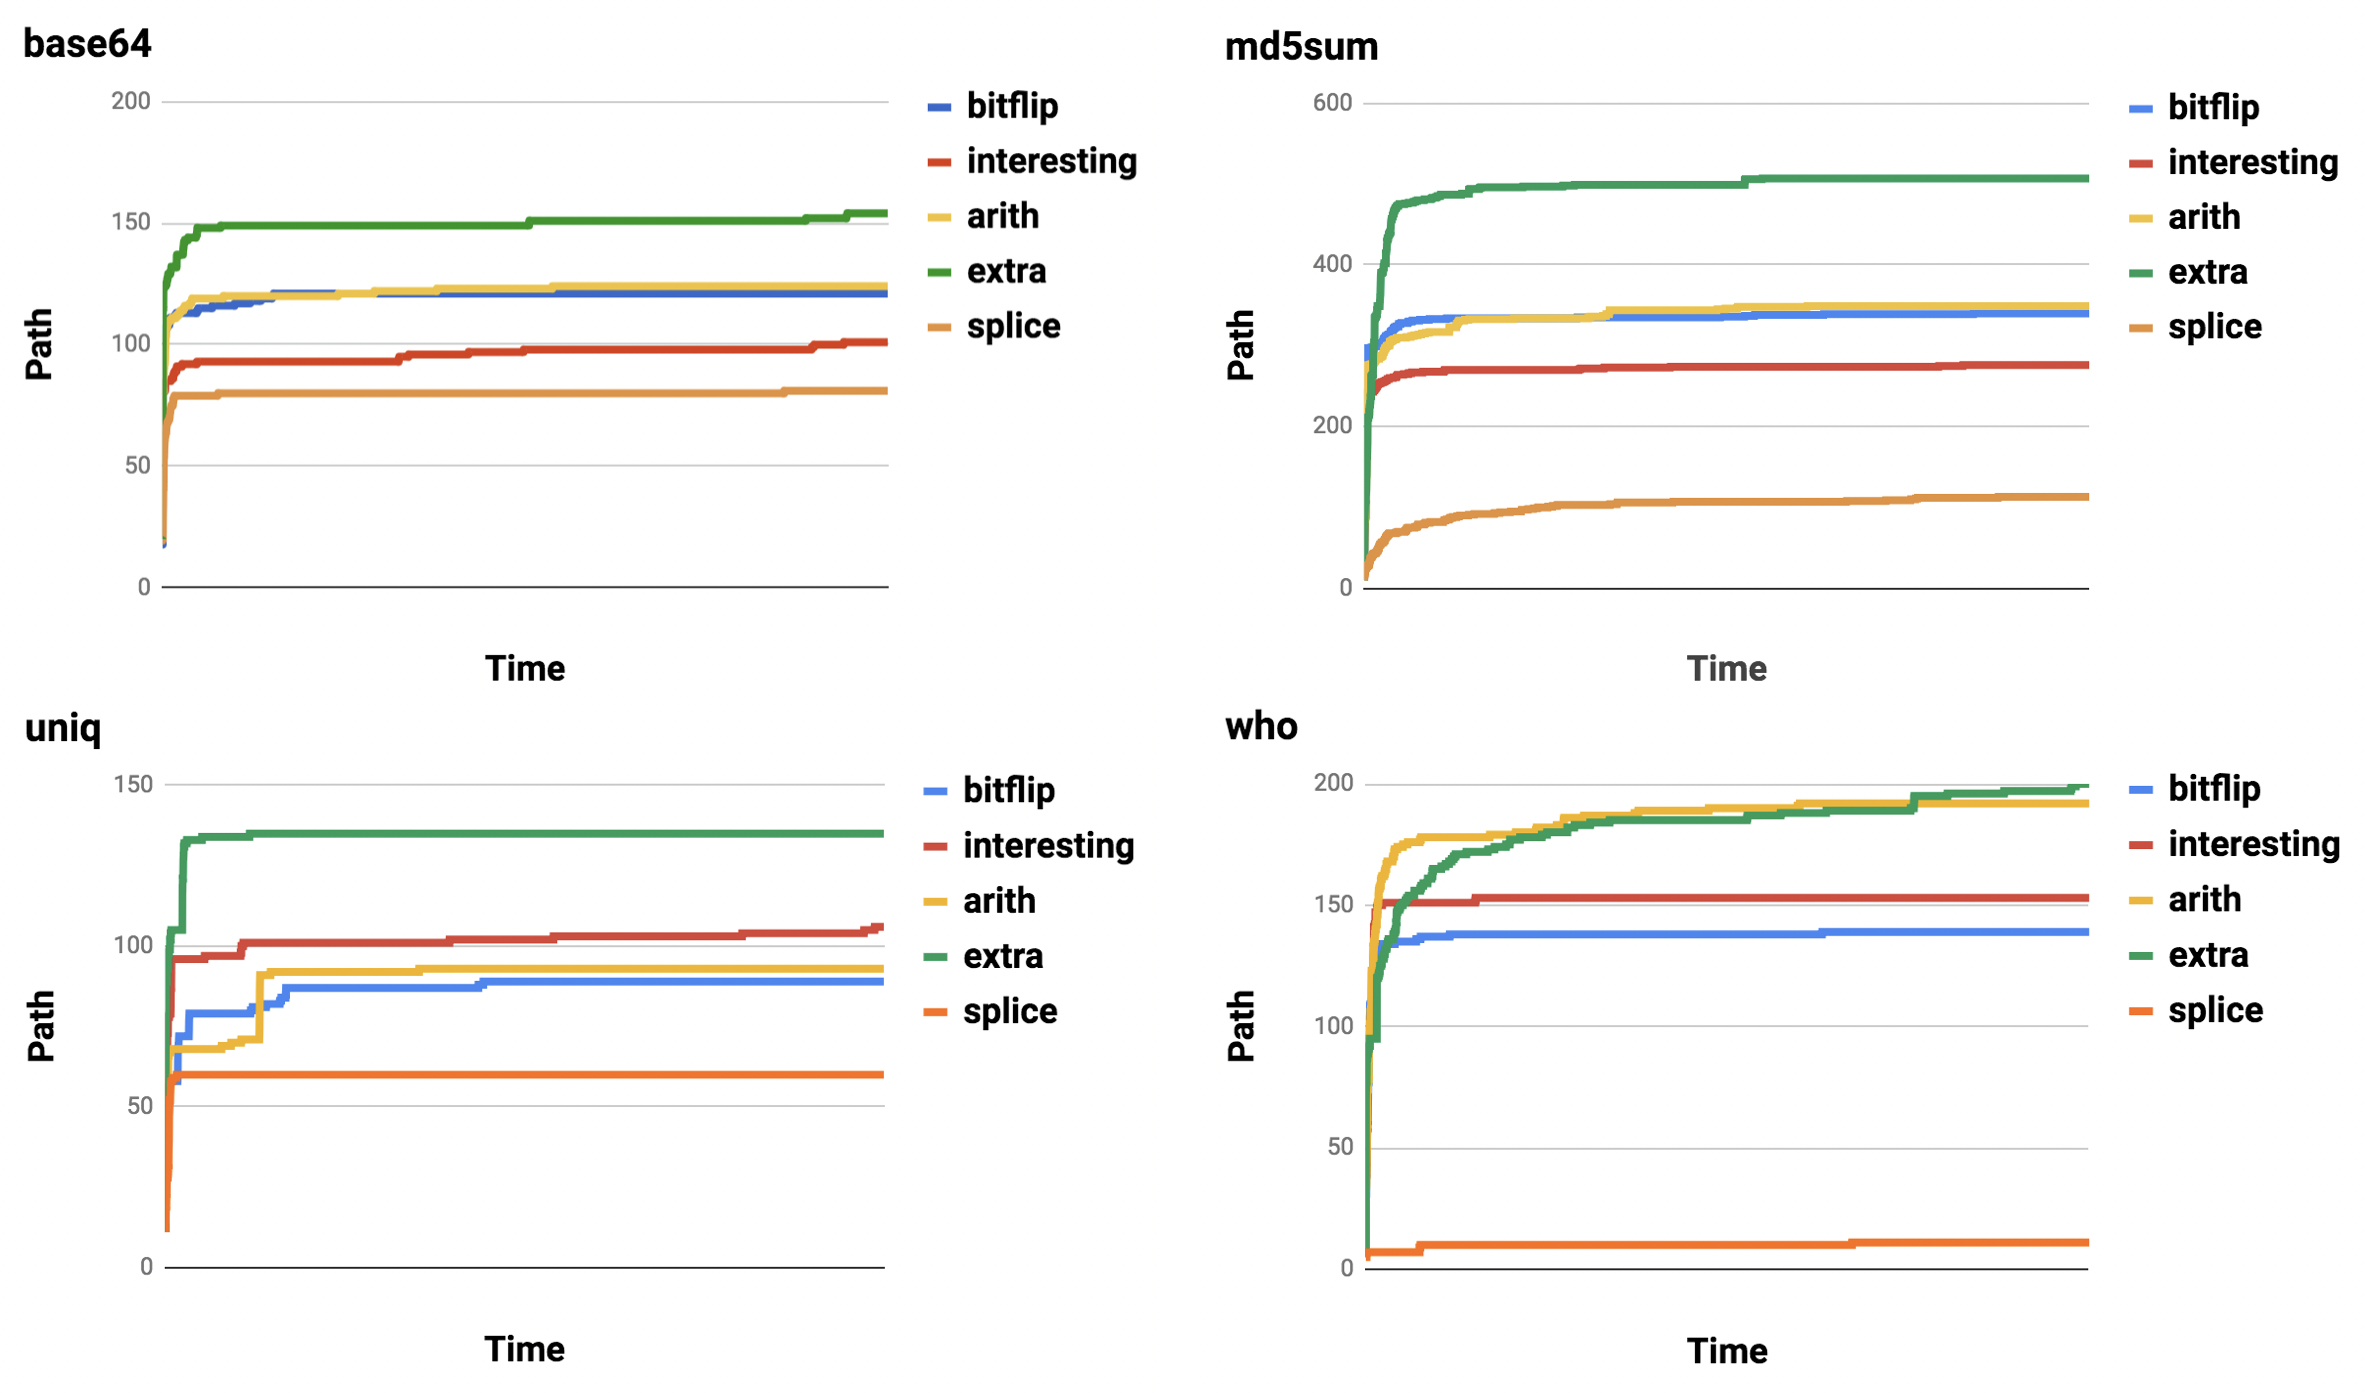
\includegraphics[width=3.6in]{pic/Mutators.png}
    \caption{Performance of Different Mutators }
    \label{Mutators}
\end{figure}

Thus, an empirical evaluation of AFL's five mainstream kinds of mutators is performed to answer above question. The statistical result on LAVA-M data set is shown in Fig.\ref{Mutators}. It indicates that (1) different kinds of mutation operators have different power for path growth; (2) extra (i.e., block-level deletion, insert and overwrite) mutation operators have better performance to help path growth, while splice mutation operators perform poor in general.

Motivated by above observation, granularity-aware scheduling of mutators is proposed. The proportion of mutation operators, which has better ability to trigger new paths (e.g., extra mutators) will be increased gradually. And over time, number of mutation operators that are chosen to applied on the seed is increased too. More specific, the scheduling algorithm for mutation operators is illustrated in algorithm \ref{schedule}.

\begin{algorithm}[h]
\caption{MutateInput(): Schedule of Mutators} 
\label{schedule}
\hspace*{\algorithmicindent} \textbf{Input}:  $s$, the seed to be mutated. \\
\hspace*{\algorithmicindent} \textbf{Input}:  $i$, the number of generated new test case.\\
\hspace*{\algorithmicindent} \textbf{Output}: $t$, the generated new test case.

\begin{algorithmic}[1]
        \STATE $\beta$= 1/ 3$^{process\_time}$;
        \STATE $p \leftarrow iteratorNum(i) * (1 -\beta)$
        \STATE $s' \leftarrow$ \texttt{RandomMutate}($s$, $p*(1-\alpha + \beta)$);
        \STATE $t \leftarrow$ \texttt{ExtraMutate}($s'$, $p * (\alpha - \beta$));
        \STATE return $t$
\end{algorithmic}
\end{algorithm}

Where $p$ represents number of selecting and applying different granularity mutation operators. The $process\_time$ refers to the execution time of fuzzing. And $\alpha$ is a constant ratio to conduct extra mutation. Over time, the $\beta$ will become smaller, and proportion of extra mutators will become higher. At the same time, $p$ becomes bigger,  and modification will become more full. In practice implementation, the $\alpha$ is set to 0.3.




\section{Implementation}\label{impl}

\begin{figure*}[tb]
\centering
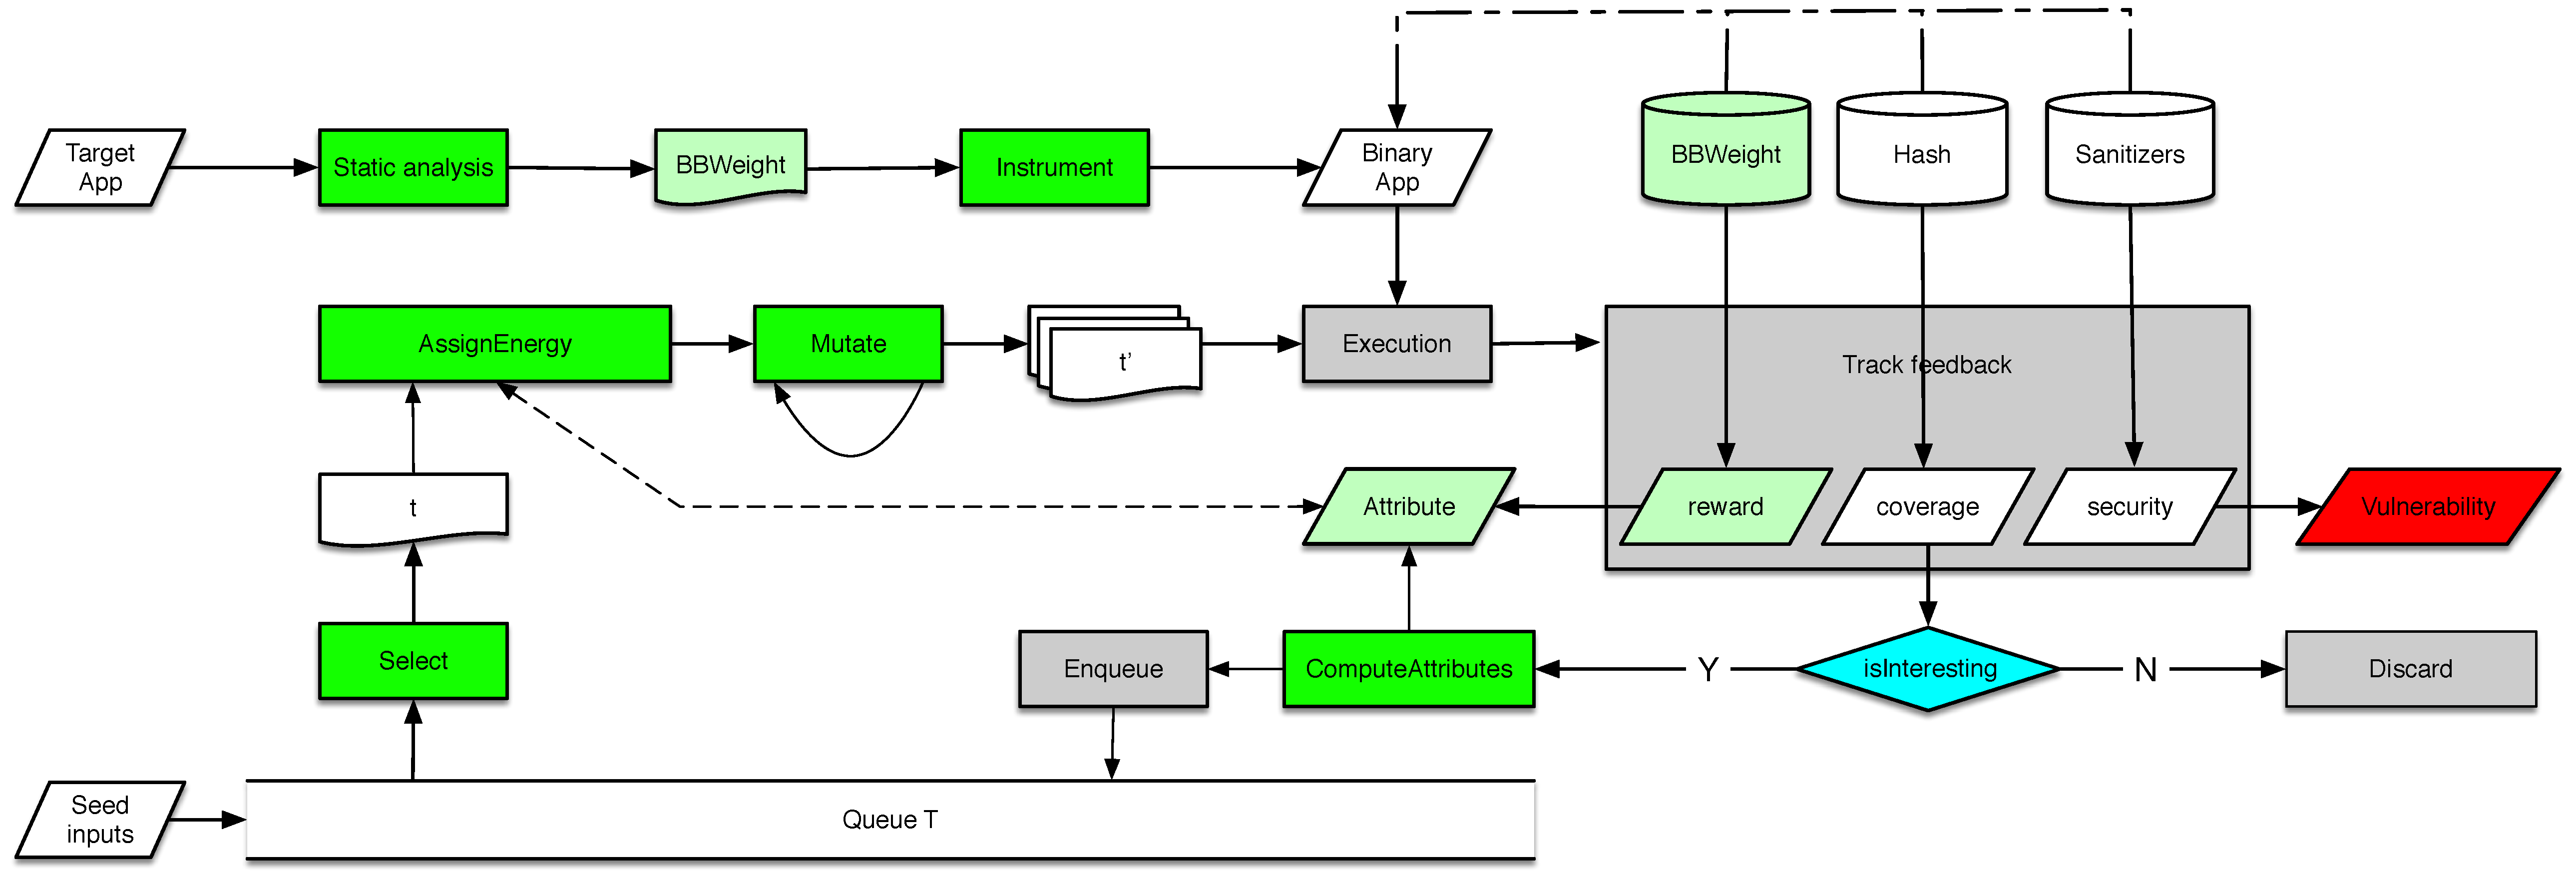
\includegraphics[width=7.2in]{pic/TAFL.eps}
\caption{Overview of TAFL}
\label{table:tafl}
\end{figure*}

We incorporate the aforementioned improvements into AFL's energy distribution, and developed a new fuzzing tool named TAFL on top of afl-2.52b. 

An overview of TAFL is illustrated in Fig. \ref{table:tafl}. Firstly, four kinds of promising vulnerable regions related metrics are extracted from a target program by static analysis. Then extracted weights of metrics are instrumented into target binary using compiler instrumentation. The reward of path exercised by a input was traced at run-time. These path rewards are used to distribute fuzzing energy, which includes phrases of selecting seed and assigning energy. TAFL prefers to select test cases that win higher rewards and assign more energy for them. The directed fuzzer strengthens fuzzing these promising vulnerable regions (i.e. sensitive regions, complex regions, deep regions and rare-reach regions). Furthermore, scheduling of mutation operators will increase the proportion of extra mutators over time, which have better ability to trigger new paths. The details of implementation are described in the following:

\subsubsection{Metric  Extraction}
Weight extraction for each metric is implemented as one LLVM pass \cite{pass}. They are used to obtain weight value of region's feature related metrics including sensitive degree, complexity, depth and rare-reach degree. These passes are used and activated by compiler afl-clang-preprocess. Each preprocess pass has a corresponding environment variable, i.e., GET\_MEM\_DENSITY, GET\_INST\_NUM, GET\_DEPTH, and GET\_ENTRY\_DEGREE. When environment variable of compiler CC is set to afl-clang-preprocess, and any of above LLVM passes' environment variable is set, related weight information of each basic block is generated and stored into a text file after the project is built.

\subsubsection{Compiler Instrumentation}
The BB weight file for each metric consists of the BB's name and its metric weight value. It is taken by compiler to instrument the weight value into target executable binary. More specifically, an extended trampoline is injected for each basic block. The trampoline is a piece of assembly code that is executed after the jump instruction, in order to keep track of the coverage control-flow edges. An edge is represented by a byte in a 64KB shared memory. On a 64-bit architecture, we extend 16 additional bytes of shared memory to record the reward feedback. 8 bytes are used to accumulate weight value, and another 8 bytes are used to record number of executed basic blocks. The instrumentation is implemented as an extension of AFL LLVM pass. When performing instrumentation, set compiler to afl-clang-fast, and compiler's flags to reference related BB weight file, then build target project.

\subsubsection{Energy Distribution}
TAFL fuzzes the instrumented executable binary with integrated energy distribution strategy. It selects seed and assigns energy based on run-time reward of test case. The current test case's reward is computed by dividing accumulated BB weight for different metrics by the number of exercised basic blocks. TAFL selects those test cases that wins higher reward and assign energy based on seed's reward factor. Besides, its implementation of MutateInput in havoc stage is modified to improve the proportion of extra mutators over time.

We have open sourced our tool which is available for download at \url{https://sites.google.com/view/tafl/tool}.
\section{Evaluation}\label{experiment}

In this section, we evaluate the performance improvements brought by TAFL using well-known benchmarks. The evaluation setup environments are firstly described, including the used benchmarks, evaluation tools, experimental infrastructure and research questions we are trying to answer. We also represent and explain our evaluation results.

\subsection{Evaluation Setup}

\begin{table*}[t]
\centering
% \begin{adjustbox}{max width=\columnwidth}
\begin{adjustbox}{max width=\textwidth}

\begin{tabular}{|l|l|l|l|l|l|l|l|l|l|l|l|l|l|l|l|}
\hline
\multirow{2}{*}{\textbf{App}} & \multicolumn{3}{l|}{\textbf{AFL}} & \multicolumn{3}{l|}{\begin{tabular}[c]{@{}l@{}}\textbf{TAFL-sen}\end{tabular}} & \multicolumn{3}{l|}{\begin{tabular}[c]{@{}l@{}}\textbf{TAFL-com}\end{tabular}} & \multicolumn{3}{l|}{\begin{tabular}[c]{@{}l@{}}\textbf{TAFL-deep}\end{tabular}} & \multicolumn{3}{l|}{\begin{tabular}[c]{@{}l@{}}\textbf{TAFL-rare}\end{tabular}} \\ \cline{2-16} 
                     &\textbf{ first(min) }  & \textbf{crash}  & \textbf{path}  & \textbf{first(min)}                   & \textbf{crash}                  &\textbf{ path }                 & \textbf{first(min)}                 & \textbf{crash                 } &\textbf{ path    }              & \textbf{first(min) }                  & \textbf{crash}                & \textbf{path}             &\textbf{ first(min)}                  & \textbf{crash}                  & \textbf{path}                  \\ \hline
base64         &   23.15  &             53              &        155              &        -34.64\%            &         +30.18\%          &         -15.48\%               &      -38.83\%              &     +28.30\%                  & -4.51\%  &          -92.74\%           &      +15\%               &       -2.5\%               & -16\%& +66\% & +87.4\% \\ \hline
md5sum             &   1.95      &    32    &  370     &       -18.22\%                  &     +21.87\%                   &  +2.43\%       &       -35.44\%     &       -12.5\%        &      -2.43\%      &        -52.91\%     &         +31.25\%   &                      +4.32\% &        -28.86\%     &          +15.62\%      &      +5.13\%      \\ \hline
uniq                    &   1072.65     &   1    &   126 &       -29.95\%            &          0\%          &     0\%                &       -7.07\%               &     0\%               &     +1.28\%                  &      -84.81\%                 &    0\%                 &       +4.76\%             &   -13.51\%       &        0\%               &     +6.34\%     \\ \hline
who                     &   937.31   &     2  &   202        &           -6.18           &       0\%           &     +7.9\%                &    -29.66\%              &       0\%            &       -7.4\%                 &          -15.37\%            &      0\%              &                     +10.89\% & +4.36\%       &   0\%    & +1.98\%            \\ \hline
libxml2-2.9.2     &   534.61      &    12    &   6080    &        -60.84\%              &     +41.66\%               &       +5.50\%                &       +20.54\%                &       -33.33\%       &+3.79\%  &     -35.90\%    &        +133.33\%  &      +7.36\%            &      -56.82\%          &         +216.66\%            &      +12.61\%                            \\ \hline
libtiff-3.7.0        &   0.08          &    52    &  469       &         0\%                  &      +21.53\%                 &       +15.35\%                &        0\%                         &     +17.30\%                  &     +10.87\%                 &          0\% &       +36.53\%   &        +11.08\%             &         0\%               &         +23.07\%              &    +15.99\%                  \\ \hline
%libtasn1-4.12      &    1318.53     &    1    &    776   &          -             &        -                &        -4.25\%               &        -                 &          -              &          -1.28\%             &        -                 &        -                &      +1.15\%                 &            -             &           -              &        +4.89\%               \\ \hline
bison-3.0.4        &  52.14       &   161     &   3591    &           -95.43\%              &       +18.01\%                 &      +8.71\%               &     -90.64\%               &    +4.96\%      & +4.42\%           &     -58.38\%        &          +31.67\%           &         +3.70\%               &     -72.13\%                &        +19.87\%              &        +29.15\%                        \\ \hline
cflow-1.5            &     22.65    &    166    &           1331                    &   -68.78\%                  &    +6.02\%                  &     -0.52\%                   &       -55.05\%              &        +44.57\%        &    +2.55\%                   &    +51.74\% &        -3.61\%             &        -0.75\%                 &         -58.41\%               &     +5.42\%      &    +0.75\%      \\ \hline
libjpeg-tubo-1.2.0   &  117.25      &   22     &   2908    &        -18.43\%         &      -18.18\%                  &      -3.25\%                 &       -53.72\%    &     +104.54\%       &         +8.70\%        &       -108.31\%                  &                       -18.18\% &         -10.24\%              &      +10.53\%                   &     -45.45\%                    &     -3.12\%                  \\ \hline
%jasper-2.0.14     &   3.45      &   283     &       &                         &                        &                       &                         &                        &                       &                         &                        &                       &                         &                         &                       \\ \hline
%ImageMagick-7.0.8    &         &        &       &                         &                        &                       &                         &                        &                       &                         &                        &                       &                         &                         &                       \\ \hline
\textbf{Average}         &     -      &   -   &  -  &\textbf{-36.94\%} & \textbf{+15.05\%} & \textbf{+2.29\% }    & \textbf{-32.21\% }& \textbf{+17.09\%} & \textbf{+1.91\%} & \textbf{-20.01\%} & \textbf{+25.12\% }& \textbf{+3.17\%} & \textbf{-28.27\%} & \textbf{+31.26\%} & \textbf{+17.39\%}  \\\hline 
\end{tabular}
\end{adjustbox}
\caption{Results of Directing Towards Four Kinds of Promising Regions}
\label{TargetAreas}
\end{table*}


\textbf{Evaluation Datasets}: A widely used benchmark (i.e., LAVA-M ) and some popular open source projects are selected for the evaluation. The programs in selected benchmarks are known to have specific vulnerabilities, and hence form a ground-truth corpus for evaluating fuzzing tools.
\begin{itemize}

   \item \textbf{LAVA-M Dataset}. LAVA-M consists of four buggy versions of Linux utilities, i.e., \texttt{base64}, \texttt{md5sum}, \texttt{uniq} and \texttt{who}. It was generated by automatically injecting known vulnerabilities into hard-to-reach regions of the source code \cite{lava}. It is commonly used as a benchmark for evaluating the capability of various fuzzing tools. The authors of recent fuzzing tools (e.g. VUzzer\cite{rawat2017vuzzer}, CollAFL\cite{gancollafl}, and Angora \cite{chen2018angora} all used this benchmark.
        
    \item \textbf{Real-World Projects}. Some popular open source Linux projects are selected, including document process libraries (e.g., libxml2), image processing libraries (e.g., libtiff) and so on. They are chosen based on the following criteria: popularity in the community, development activeness, and diversity of categories.  
\end{itemize}


\textbf{Evaluation Tools}: AFL based greybox fuzzing is our focus. Thus AFL and its variants based on source level instrumentation are our comparison targets.  Furthermore, we only select tools that are available for download online. These tools include:
    
\begin{itemize}

    \item \textbf{AFL-2.52b}:  It is the latest version of official AFL.
    
    \item \textbf{AFLFast}: It is an AFL variant that tries to balance the energy distribution by spending more energy on low-frequency path.
    
    \item \textbf{FairFuzz}: It is an AFL variant that guides the fuzzer to approach rarely reached branches.
    
    \item \textbf{TAFL}: It is our extension of AFL, which is integrated with improvements of directing towards four kinds of promising vulnerable regions and granularity-aware scheduling of different kinds of mutation operators. 
\end{itemize}


\textbf{Experimental Infrastructure}: Fuzzing tools are evaluated on collected benchmarks with the same configuration, i.e., a virtual machine configured eight core of 2GHz Intel CPU and 8 GB RAM, running Ubuntu 16.04.


\textbf{Research Questions}: We evaluated each improvement and integrated performance of TAFL, and try to answer the following research questions:

\begin{itemize}

    \item \textbf{RQ1:} The effectiveness of directing towards four kinds of vulnerability promising areas.
    
    \item \textbf{RQ2:} The effectiveness of scheduling of different mutation operators.
    
    \item \textbf{RQ3:} The performance of integrated TAFL compared with existing mainstream AFL based greybox fuzzers.
    
\end{itemize}



\subsection{Evaluation of Directing Towards Promising Regions}
\label{sec:directing}
The effectiveness of directing fuzzers toward four kinds of promising regions that are more likely for a vulnerability to reside are evaluated. Furthermore, we compare the results with the  original AFL. Note that TAFL used in this evaluation is only integrated with improvement of guidance, without scheduling of mutators. Each project is executed ten times for 24 hours in order to reduce the random noise of fuzzing. Results are collected and illustrated in Table \ref{TargetAreas}. 
In the table, the four directed fuzzing strategies are donated as \textit{TAFL-sen} (sensitive region),  \textit{TAFL-com} (complex region), \textit{TAFL-deep}  (deep region) and \textit{TAFL-rare}  (rare-reach region) respectively.
Three measurement metrics, including time to trigger the first crash, total unique crashes and total paths are used. They are labeled as \textit{first}, \textit{crash} and \textit{path} respectively in the table.
 % are used to show the effectiveness and performance of four kinds of promising vulnerable regions guided search strategies.
\subsubsection{First Blood }

Time to trigger the first crash is an important factor to evaluate a directed fuzzing tool. As we could see from Table \ref{TargetAreas}, all the four directed fuzzing strategies advance the time to find the first crash in most cases. The average advance ratio for detecting first blood are 36.94\%, 32.21\%, 20.91\%, 28.27\% for four kinds of area directed strategies respectively. Generally speaking, sensitive regions guided fuzzing has better performance of triggering the first crash on selected benchmarks. In some specific cases like bison-3.0.4, sensitive area directed strategy brings 95.43\% performance improvement. This result proves that if a code region contains more memory and string related instruments, it has more chances to occur memory corruption problems.

\subsubsection{Unique Crashes}
Another important characteristic of a good fuzzers is its ability to find unique crashes in limited time. Although the same root crash may cause multiple unique crashes, and some are even not exploitable, in general, more unique crashes indicate better chances to find vulnerabilities. 
% In AFL, different paths to the same crash point are marked as separate unique crashes. Thus unique crashes metric also show the explored degree of vulnerable point. The total crashes could indirectly prove effectiveness of improvement of guidance. 
As can be seen from Table \ref{TargetAreas}, four regions directed strategies get more unique crashes in most cases, and average improvements are 15.05\%, 17.09\%, 25.12\%, 31.26\% respectively. The results prove the effectiveness of improvement in directing fuzzing toward promising areas. Moreover, among four kinds of region directed strategies, rare-reach region directed strategy performs the best in general. Especially, its improvement reaches 216.66\% in the case of libxml2-2.9.2. It proves that regions without sufficient testing may have higher probabilities for a vulnerability to reside.

\subsubsection{Total Paths}
Another important factor is the number of total paths a fuzzer can traverse in limited time. For four vulnerable region directed strategies, the average improvements are 2.29\%, 1.91\%, 3.17\% and 17.39\% respectively. The result shows that rarely reachable region guided strategy is much more helpful to path growth. Furthermore, we could conclude from the above results that the strategy of directing fuzzing towards rarely reachable regions outperform all the other on selected benchmarks.



\subsection{Evaluation of Scheduling of Different Mutators}
Code coverage is one of the critical factors for fuzzers' success. 
% It is also the most important metric to show performance of different distribution strategies of various mutation operators. 
We use two coverage related metrics (i.e., path growth over time and total reachable paths) to validate the effectiveness of our improvement to mutator scheduling. The evaluation was performed on collected benchmarks, and each project ran ten times for 24 hours for the sake of reducing fuzzing's random noise. The result is counted and illustrated in Table \ref{EffectiveOfMutatorDistribution}.

\subsubsection{Path Growth Over Time}
Path growth over time is a direct indicator of fuzzer's ability to explore new paths. The original AFL and AFLFast are modified to add improvement of scheduling for different mutation operators. Due to limited space of the article, we selected partial results to illustrate the effectiveness of scheduling of mutation operators in Fig. \ref{mutateSchedule}. For more empirical results, please refer to our website (\url{https://sites.google.com/view/tafl}).

\begin{figure}[t]
    \centering
    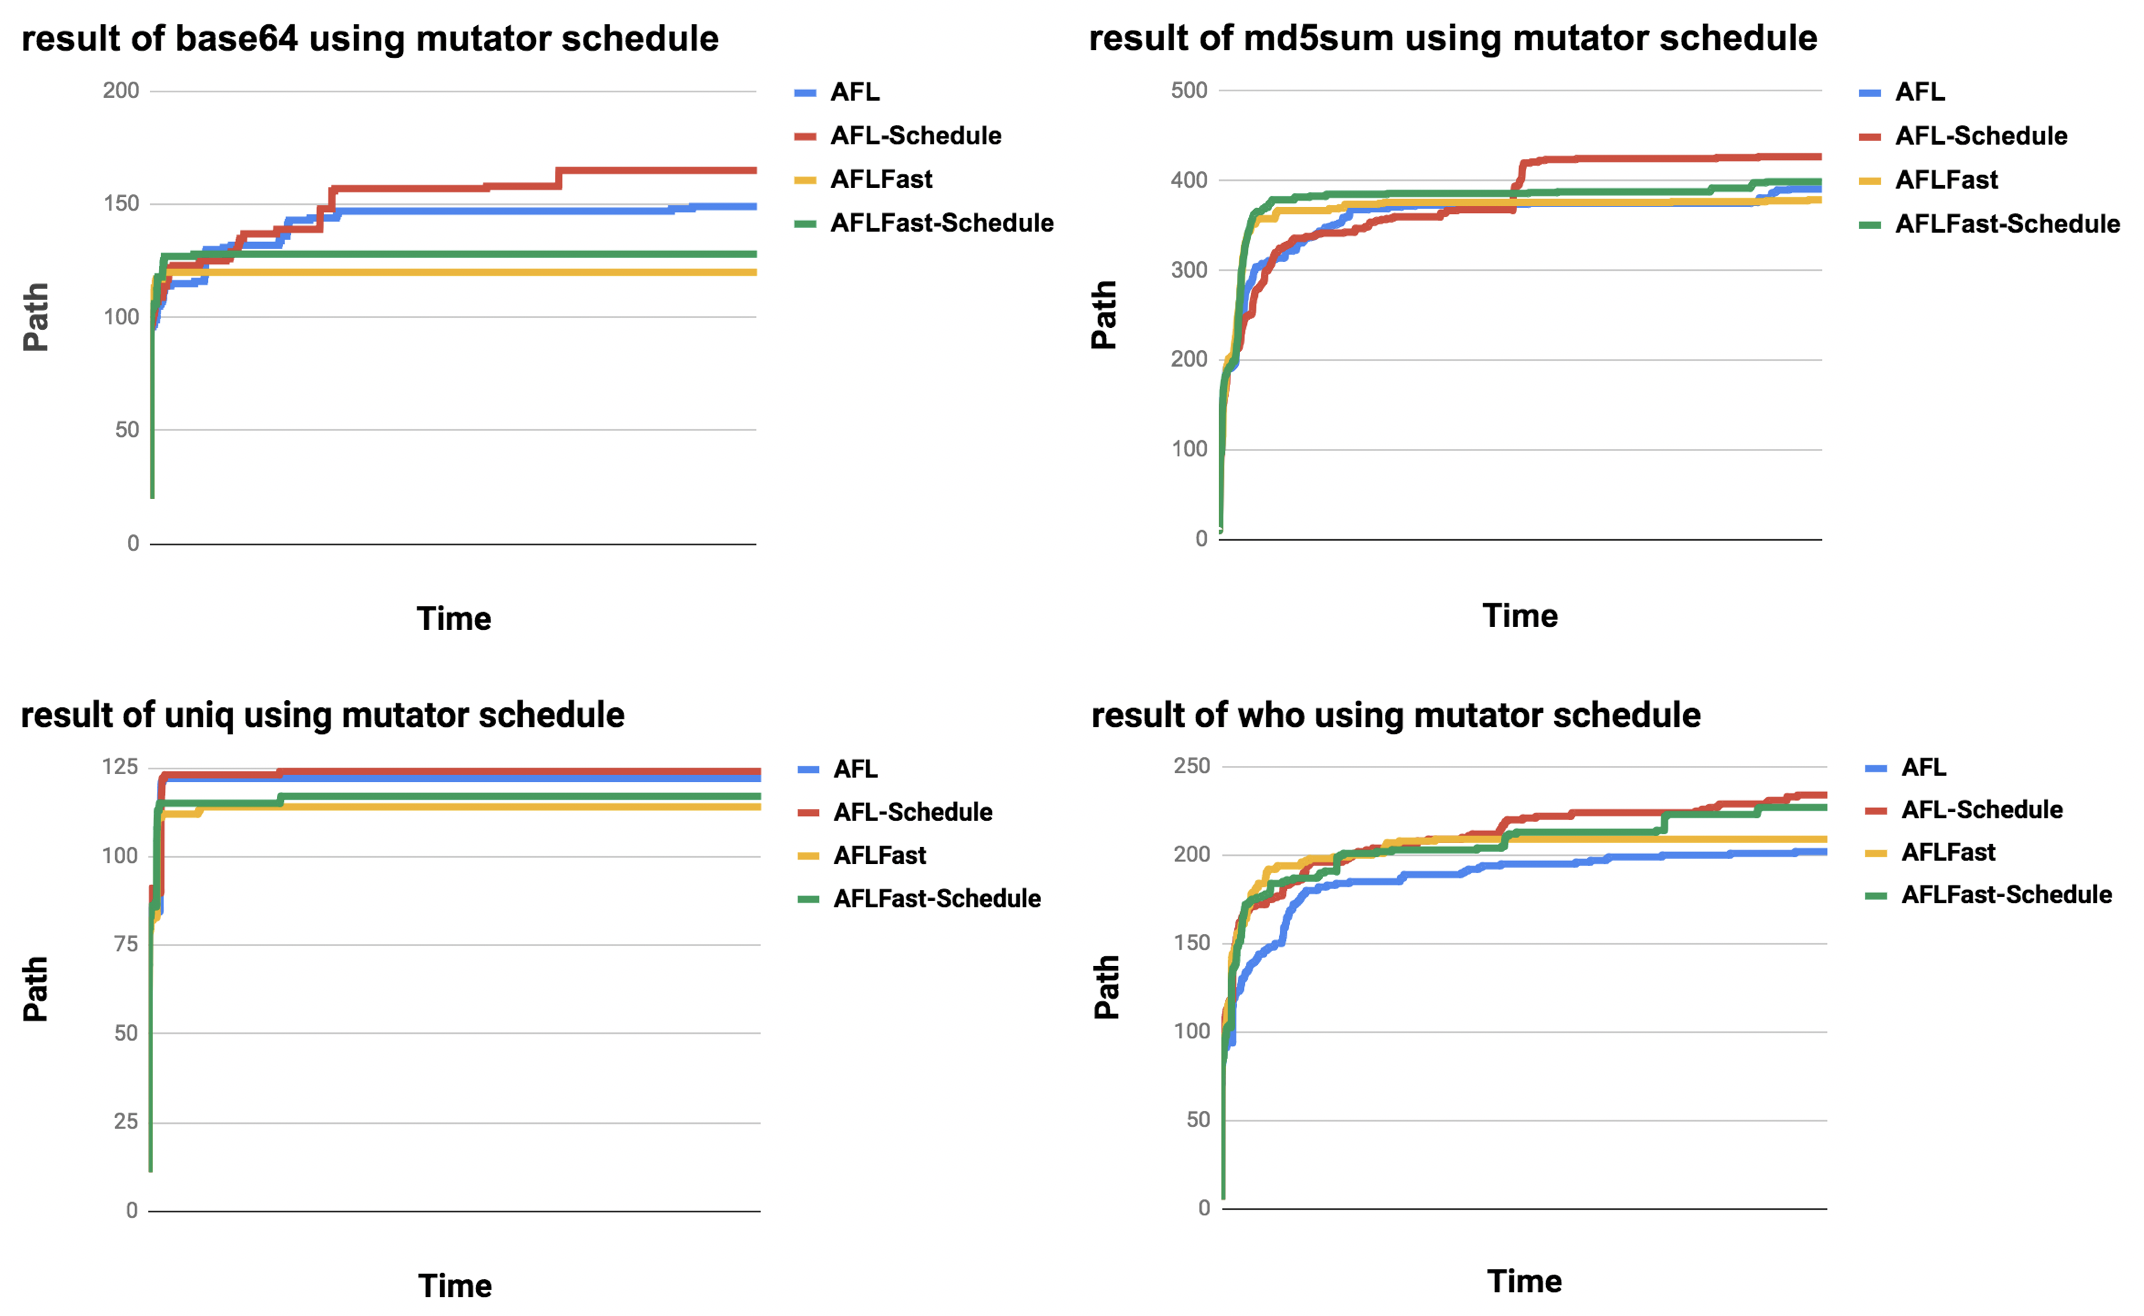
\includegraphics[width=\columnwidth]{pic/scheduleLAVM12.png}
    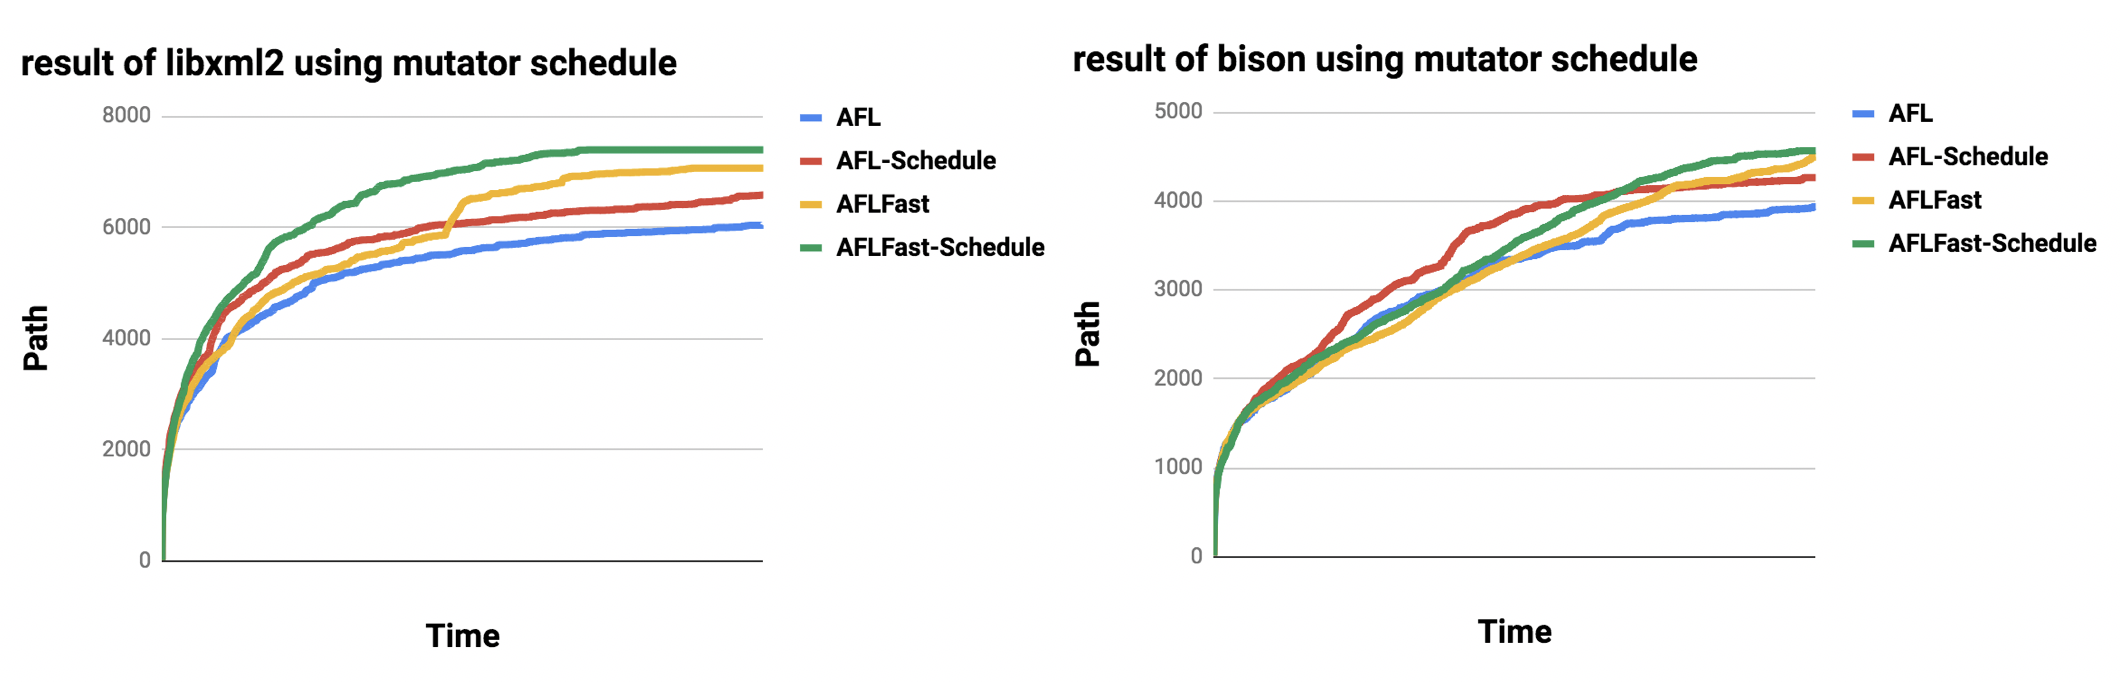
\includegraphics[width=\columnwidth]{pic/schedule22.png}
    \caption{Results of Scheduling Mutators}
    \label{mutateSchedule}
\end{figure}

As can be seen from above Fig.\ref{mutateSchedule}, fuzzers with scheduling of mutators could trigger new paths more quickly than than those without scheduling in most cases. Scheduling of mutators is helpful to maximize code coverage in limited time. The results prove the effectiveness of scheduling mutators. Besides, we observe that AFLFast is better than AFL in most cases within 24 hours. However, in some case such as base64, AFLFast's performance is worse than AFL. In practice, AFLFast's will slow down to zero after a specific time. The reason is that low-frequency paths in base64 are time-consuming, which stuck AFLFast.

\subsubsection{Improvement of Total Path}

\begin{table}[t]
\centering
\begin{adjustbox}{max width=\columnwidth}
\begin{tabular}{|l|l|l|l|l|}
\hline
\textbf{Application }      & \textbf{AFL} & \textbf{AFL-schedule} & \textbf{AFLFast} & \textbf{AFLFast-Schedule} \\\hline
base64            &   155 &  +10.7\%     &    120     &    +6.6\%              \\ \hline
md5sum          &   370 &    +5.2\%    &      378   &      +8.9\%            \\ \hline
uniq                 &  126   &   +3.2\%     &   114      &     +2.6\%              \\ \hline
who                  &  201   &  +15.8\%      &   219      &    +8.6\%            \\ \hline
libxml2-2.9.2   & 6080   &   +14.7\%      &  6402       & +13.9\%        \\ \hline
libtiff-3.7.0       &  469   &   -0.9\%     &      514   &       +2.5\%          \\ \hline
bison-3.0.4       &  3591   &      +9.4\%        &   4324      &   +4.7\%      \\ \hline
cflow-1.5           & 1331    &   +1.6\%     &   1294      &  +2.7\%               \\ \hline
libjpeg-tubo-1.52 & 2908    &    +3.6\%    &   3087      &   +1.3\%         \\ \hline
\textbf{Average}               &   -  &   \textbf{+7.03\%}    &    -      &     \textbf{+4.82\% }                \\ \hline
\end{tabular}
\end{adjustbox}
\caption{Paths Improvement of Scheduling Mutators}
\label{EffectiveOfMutatorDistribution}
\end{table}


Furthermore, we show the total executed paths by AFL, AFLFast and their improved versions in Table \ref{EffectiveOfMutatorDistribution}.
Scheduling of mutators is useful to improve code coverage in most cases. For AFL and AFLast, the average increased percentage on selected benchmarks are 7.03\% and 4.82\% respectively. In certain cases such as libxml2-2.9.2, the promotion percentage could be as high as 15.8\% and 14.7\%. In some lousy cases such as libtiff-3.7.0, the ratio could drop to -0.9\%. We observe that the the difference of different fuzzing strategies' efficiency are obvious when limited time is given. If enough time is given, the eventual discovered paths will be very close for different fuzzing strategies. This is because all the easily reachable regions are already explored.

\subsection{Evaluation of Integrated Performance}
In this section, we evaluate the overall performance of TAFL compared with AFL, AFLFast and FairFuzz, which means TAFL is integrated with the capability to direct towards promising regions and
to schedule of different mutators. Similar to Section~\ref{sec:directing}, the same set of metrics are used to measure the performance. Each project is fuzzed ten times for 24 hours in order to reduce the random noise of fuzzing, and the results are collected and illustrated in Table \ref{Integration}.


\begin{table*}[t]
\centering
% \begin{adjustbox}{max width=\columnwidth}
\begin{adjustbox}{max width=\textwidth}
\begin{tabular}{|l|l|l|l|l|l|l|l|l|l|l|l|l|}
\hline
\multirow{2}{*}{\textbf{App}} & \multicolumn{3}{l|}{\textbf{AFL}} & \multicolumn{3}{l|}{\textbf{AFLFast}} & \multicolumn{3}{l|}{\textbf{FairFuzz}} & \multicolumn{3}{l|}{\begin{tabular}[c]{@{}l@{}}\textbf{TAFL-rare}\end{tabular}} \\ \cline{2-13} 
                             &\textbf{ first  blood   }        &\textbf{ crashes }    &  \textbf{paths}     &\textbf{ first blood  }          & \textbf{crashes }   & \textbf{paths }     &\textbf{ first  blood  }     &  \textbf{crashes }   & \textbf{ paths }       &\textbf{ first blood }              &\textbf{ crashes }        &\textbf{ paths }                              \\ \hline
base64               &  23.15          &    53       & 155     &     59.46     &    52       &   139        &   0           &      0       &    134     &      20.3          &       83          &         288                          \\ \hline
md5sum            &    3.95           &    32       & 370    &    2.13         &    37       &    378       &   5.81      &    30       &     301    &      3.23           &       43          &        412                         \\ \hline
uniq                   &    1072.65     &   1           & 126    &    901.01     &    1          &  132          &  0            &     0        &    134     &      717.19        &       1             &        144                          \\ \hline
who                   &    937.31       &    2          & 202   &  890.33      &    2          &  209         &  0            &     0        &     206    &     915.54      &       2             &         216                         \\ \hline
libxml2-2.9.2    &   534.61        &    12    &  6080   &    560.23     &     17       &  6402       &  826.7    &     22      &   6410    &     330.81       &      41            &        7331                        \\ \hline
libtiff-3.7.0       &     0.08          &   52    &    469   &      0.08        &   52        &    512         &  0.08      &     62    &   490       &     0.08           &      68            &       571                         \\ \hline
%libtasn1-4.12    &    1318.53      &    1      &    776   &                      &               &                &                 &              &                 &                                  &                    -       &                                          \\ \hline
bison-3.0.4      &   52.14            &    161 &   3591  &    42.23        &  208       &   4324    &    5.68     &  119       &  3214       &     19.53          &    196           &        4709                        \\ \hline
cflow-1.5          &   22.65           &    166  &   1331   &    5.81        &      177    &    1321    &     33.52   &    204   &   1197        &     7.42            &    173           &        1412                         \\ \hline
libjpeg-tubo-1.2.0   &   117.25   &    22    &   2908    &   58.5       &      12    &    3087    &   786.03   &    4      &    1681       &     85.91          &    12             &        2978                       \\ \hline
%jasper-2.0.14        &         &        &       &          &          &        &          &          &         &                         &                        &                       &                         &                        &                       &                         &                        &                       &                         &                         &                       \\ \hline
%ImageMagick-7.0.8    &         &        &       &          &          &        &          &          &         &                         &                        &                       &                         &                        &                       &                         &                        &                       &                         &                         &                       \\ \hline
Average  &    337.08           &     55.66      &    1692.44       &      279.97             &    62         &   1833.77            &      276.34       &    49      &    1529.66           &     248.18        &      68.77          &         2006.78 \\ \hline
\textbf{Improvement}  &    -                     &     -               &    -                   &    \textbf{ -16.94\% }           &\textbf{+11.39\%  }         &  \textbf{ +8.35\% }         &    \textbf{  -18.01\%}       &    \textbf{-11.97\%}        &    \textbf{-9.62\%}            &  \textbf{-26.37\%}      &   \textbf{+23.55\% }    &  \textbf{+18.57\% }             \\ \hline
\end{tabular}
\end{adjustbox}
\caption{Comparison Results of TAFL and AFL based Greybox Fuzzers}
\label{Integration}
\end{table*}

\subsubsection{First Blood}
As is shown in Table \ref{Integration}, the integration of improvements is effective to advance the time to trigger the first crash. In general, the time to trigger the first crash is advanced 26.37\% after using mutator schedule. This is better than AFLFast and FairFuzz.% In general, the time to trigger the first crash is advanced by 26.37\% in TAFL after using mutator schedule.

\subsubsection{Unique Crashes}
As can be seen from the Table \ref{Integration}, compared to AFL and its extension AFLFast, TAFL-rare detects more crashes within 24 hours on selected benchmark. The improvements in total crashes of AFLFast and TAFL- rare are 11.39\% and 23.55\%. TAFL-rare is twice as many as AFLFast. Meanwhile, FairFuzz performs poor, especially on LAVA-M benchmark, it cannot detect crashes in base64, uniq, and who programs, but it could get a better result on the cflow-1.5 project.
%TAFL-rare detects more crashes within 24 hours on selected benchmark. The improvements to AFLFast and TAFL-rare are 11.39\% and 23.55\% respectively. Meanwhile, FairFuzz performs poorly, especially on LAVA-M benchmark. It cannot detect crashes in \texttt{base64}, \texttt{uniq}, and \texttt{who} programs, but it could get a better result on the cflow-1.5 project. 

\subsubsection{Total Paths}
As can be seen from the Table \ref{Integration}, the promising regions directed and mutator schedule strategy are helpful to improvement on the entire path. On the selected benchmarks, TAFL-rare brings an average improvement of 18.57\%, while the average improvements to AFLFast and FairFuzz are 8.35\% and -9.62\% respectively. Furthermore, TAFL helps us find five unknown bugs and identify one new CVE\cite{bugs}. 
%The combination of the two strategies is helpful to the improvement on the entire path. On the selected benchmarks, TAFL-rare brings an average improvement of 18.57\%, while the average improvements to AFLFast and FairFuzz are 8.35\% and -9.62\% respectively. Furthermore, TAFL helps us find five unknown bugs and identify one new CVE\cite{bugs}. 


\section{Related Work}\label{relatedwork}
% Researchers have done a lot of work to improve AFL's capabilities, which could be categorized into three directions:

We review related work that improves AFL's capabilities from three dimensions.

(1) \textbf{Effectiveness:} Effectiveness concerns about meta-abilities of fuzzers to bypass obstacles and trigger vulnerabilities. Generally speaking, there are three approaches to improving effectiveness. %as (1) feedback accuracy \cite{gancollafl} and granularity \cite{li2017steelix}; (2) smart mutate strategies ( i.e. where and what to mutate) \cite{zhang2018ptfuzz}  \cite{chen2013angora};  (3) sensitive to security violation \cite{serebryany2012addresssanitizer} \cite{stepanov2015memorysanitizer} and so on.
% as follows:

%\textbf{Improvement of  effectiveness}, detailed improvement could be concluded as some aspects as follows: 

\begin{itemize}

\item  \textit{Feedback granularity and accuracy:} Steelix \cite{li2017steelix} instruments AFL to collect mutate progress for magic bytes compassion, and continue to mutate on input that has progressed for each bit. CollAFL \cite{gancollafl} demonstrates that inaccuracy of feedback (i.e., hash collision issue) in AFL would limit the effectiveness of discovering path. The authors design an algorithm to resolve the hash collision problem, and improve the edge coverage accuracy with a low-overhead instrumentation scheme.  

\item \textit{Smart mutation strategy:} The mutate strategy answers the questions about where to mutate and what to mutate. To answer the former, Lin et al.\cite{lin2008convicting} propose a solution to identify raw bytes to mutate using static data lineage analysis. A deep neural network solution is proposed in \cite{rajpal2017not} to predicate which bytes to mutate. To answer the latter, Vuzzer \cite{rawat2017vuzzer} uses dynamic analysis to infer exceptional values (e.g., magic numbers to use for mutating.) 

\item \textit{Sensitive to security violation:} Fuzzers usually use program crashes as an indicator of vulnerabilities, because they are easy to be detected even without instrumentation. However, programs do not always crash when a vulnerability is triggered, e.g., when a padding byte following an array is overwritten. Researchers have proposed several solutions to detect various kinds of security violations. For example, the widely used AddressSanitizer\cite{serebryany2012addresssanitizer} and MemorySanitizer\cite{stepanov2015memorysanitizer} could detect buffer overflow and use-after-free vulnerabilities. There are many other sanitizers available, including UBSan\cite{lee2015type}, DataFlowsanitizer \cite{DataFlowSanitizer}, ThreadSanitizer \cite{serebryany2009threadsanitizer} and so on.
\end{itemize}



(2) \textbf{Efficiency:} Efficiency concerns about improving code coverage in order to improve the probability of trigger more vulnerabilities. Previous efforts were conducted following three approaches.% like (1) providing high quality and diversity of intial seeds \cite{wang2017skyfire} \cite{godefroid2017learn} \cite{nichols2017faster} \cite{lv2018smartseed}; (2) Improving the execution speed by prioritize faster and smaller seed, using new primitives \cite{xu2017designing} and utilizing system fork mechanism and hardware features (e.g Intel-PT) \cite{schumilo2017kafl} \cite{zhang2018ptfuzz}; (3) Balance the fuzzing energy distribution like low frequnce path, untouched path deserve more enery \cite{bohme2016aflfast}  \cite{gancollafl}.
% as follows:


%\textbf{Improvement of efficiency}, detailed improvement could be concluded as some aspects as follows: 

\begin{itemize}

\item  \textit{Quality and diversity of initial seeds:} Skyfire \cite{wang2017skyfire} learns a probabilistic context-sensitive grammar from abundant inputs to guide seed generation. Learn \& input \cite{godefroid2017learn} utilizes recurrent neural network(RNN) solution to generate valid seed files and could help generate inputs to pass format checks. Nicole Nichols et al.~\cite{lv2018smartseed} proposed a generative adversarial network(GAN) solution to argument the seed pool with extra seeds.
 % showing another promising solution.

\item  \textit{Execution speed:} AFL utilizes fork mechanism of Linux to accelerate the execution speed. It further uses forkserver mode and persistent mode to reduce the overhead of the fork operations. Besides, AFL prioritizes seeds that are executed faster, and thus it is likely that more test cases could be tested in a given time. Moreover, AFL also supports parallel mode, which enables multiple fuzzer instances to collaborate with each other. kAFL\cite{schumilo2017kafl} and PTfuzzer\cite{zhang2018ptfuzz} use hardware features (i.e., Intel PT) to accelerate the execution speed. Wen Xu et al. proposes several new primitives \cite{xu2017designing} which speed up AFL by 6.1x to 28.9x. 
 
\item \textit{Balance of fuzzing energy distribution:} AFLFast \cite{bohme2016aflfast} prioritizes seeds that were exercising less-frequent paths. Thus it is more likely that cold paths could be tested thoroughly and less energy will be wasted on hot paths.
% in order to balance the energy on the cold and hot paths. 
FairFuzz \cite{fairfuzz} spends more energy on less reachable branches. CollAFL\cite{gancollafl} prioritizes seeds that hit more untouched neighbors to improve the possibility to cover more new paths.
\end{itemize}


(3)  \textbf{Guidance:} The guidance criteria directs a fuzzer to focus on a specific goal. %Typical,  AFLGo \cite{bohme2017aflgo} directed fuzzing to reach some specific location as soon as possible.
%\textbf{Improvement of directiveness} directed grey box fuzzing be modeled as an object optimizing problem, detailed improvement work are including:
Along this direction, several works have been proposed.
% Detailed improvement works are including:
\begin{itemize}
\item \textit{Directing for specific locations:} AFLGo \cite{bohme2017aflgo} uses distance metrics to direct fuzzing to trigger and reproduce vulnerabilities in the specific location by giving the target locations at priority.

\item \textit{Directing for specific kinds bugs:} SlowFuzz \cite{petsios2017slowfuzz} prioritizes seeds that use more resources (e.g., CPU, memory, and energy), and try to increase the probability of triggering algorithmic complexity vulnerabilities. 
\end{itemize}

\section{Conclusion}\label{conclusion}

% We leverage two new insights to improve existing AFL's fuzzing energy distribution in a principled way. We direct fuzzer to stress fuzzing toward regions that are more likely for a vulnerability to reside based on static semantic metrics of target program. More specifically, four kinds of promising vulnerable regions (i.e., sensitive, cpmplex, deep and rare-to-reach regions) directed fuzzing are evaluated. And a granularity-aware scheduling of distribution proportion of different mutation operators is proposed. The ratio of mutation operators is increased gradually, if they have better ability to trigger new paths. All improvements are integrated and implemented into an new open source fuzzing tool named TAFL. Large-scale experimental evaluations have shown effectiveness of each improvement and performance of integration. Furthermore, TAFL helps us to find five unknown bugs and get one CVE in Libtasn1-4.13.




We leverage two new insights to improve AFL's fuzzing energy distribution in a
principled way. First, intuition suggests that four kinds code regions (i.e.,
sensitive, complex, deep and rare-to-reach regions) are more likely to contain
vulnerabilities. Therefore, we use static analysis to obtain semantic metrics
of the target program, and then direct the fuzzing tool to stress on such
regions. Second, existing energy distribution strategies randomly select mutators.
Since fine-grained mutators and coarse-grained mutators have their own advantages and
disadvantages, we can dynamically adjust the ratio of a kind of mutators if they perform better.
This results in a new granularity-aware energy distribution scheduling strategy.
These improvements have been incorporated into AFL, leading to a new fuzzing
tool named TAFL.  To show the power of TAFL, we have conducted large-scale
experiments on popular benchmarks and real-world programs. The
result is promising. Not only does TAFL outperform existing AFL and AFL
variants regarding effectiveness, but also it helps us locate five unknown
bugs and identify a new CEV in Libtasn1-4.13.

\input{texfile/8_Acknowledgement}


%ACKNOWLEDGMENTS are optional
%\section{Acknowledgments}
%The work is supported by National Natural Science Foundation of China (No.). 



\bibliographystyle{sty/IEEEtranS}
% argument is your BibTeX string definitions and bibliography database(s)
\bibliography{bib/reference}


\end{document}


